\section{Implementierung}
\label{sec:Implementation}

% Ziel: 6-8 Seiten
% Inhalt: Demo-Werk, Master Creator Architektur, Validierung

\subsection{Demo-Werk: Synthetische Konfiguration}
\label{sec:DemoWerk}

Als Demonstration und Validierungsbasis wurde eine synthetische Produktionskonfiguration für ein fiktives Werk in der Lack- und Farbenindustrie entwickelt. Das Demo-Werk simuliert die realistische Produktion von Pigmentpasten und dient als Referenzimplementierung für die entwickelten Artefakte.\\

\noindent Folgende Produktionen wurden modelliert:

\begin{itemize}
    \item \textbf{WP-1000:} Weiße Pigmentpaste (1155,5 kg Batch)
    \item \textbf{RP-1000:} Rote Pigmentpaste (1155 kg Batch)
    \item \textbf{BP-1000:} Blaue Pigmentpaste (1155 kg Batch)
\end{itemize}

\noindent Der Produktionsprozess umfasst 7 sequenzielle Schritte mit unterschiedlichen Maschinenressourcen und Prozesszeiten, die sich an etablierten Prozessketten der Lackproduktion orientieren \citep{goldschmidt:lackproduktion2019}. Besonders hervorzuheben ist die Integration einer Reinigungslogik: Materialien mit der Eigenschaft \url{IsCleaningMaterial=true} werden ausschließlich im Reinigungsschritt verarbeitet. Alle anderen Materialien laufen durch die regulären Produktionsschritte.

\paragraph{Mengenabhängige Vorgabezeiten}

Drei der sieben Prozessschritte (Dosieren, Filtration, Abfüllen) weisen mengenabhängige Bearbeitungszeiten auf, die nach dem Prinzip der linearen Zeitfunktion modelliert wurden. Die Zeitbausteine folgen dem REFA-Standard \cite{REFA2012}, während die produktionslogistische Verknüpfung von Materialmengen und Ressourcenbedarf auf \cite{guenther:produktion2020} basiert:

\begin{equation}
t_{process} = \frac{Q_{Batch} \cdot 1\,\text{s}}{1\,\text{kg}}
\label{eq:mengenabhaengig}
\end{equation}

wobei:
\begin{itemize}
    \item $t_{process}$ = Bearbeitungszeit des Prozessschritts in Sekunden
    \item $Q_{Batch}$ = Gesamtmenge der zugewiesenen BOM-Items (\url{TotalQuantityOfAssignedBomItems}) in kg
\end{itemize}

\noindent Diese Formel bildet das Verhalten von Prozessschritten ab, deren Dauer proportional zur verarbeiteten Menge ist. Für eine typische Charge von 1155 kg (z.\,B. WP-1000) ergibt sich somit:

\begin{itemize}
    \item Dosieren: $t = 1155\,\text{kg} \cdot 1\,\frac{\text{s}}{\text{kg}} = 1155\,\text{s} \approx 19,25\,\text{min}$
    \item Filtration: $t = 1155\,\text{s} \approx 19,25\,\text{min}$
    \item Abfüllen: $t = 1155\,\text{s} \approx 19,25\,\text{min}$
\end{itemize}

\noindent Im Gegensatz dazu verwenden die Schritte Mischen, Rühren und Dispergieren konstante Bearbeitungszeiten (2100s, 600s, 1800s), da deren Dauer primär von physikalischen Prozessanforderungen (z.\,B. Homogenisierungsgrad, Partikelgrößenverteilung) und weniger von der absoluten Menge abhängt. Der Maschinenführer hat offenbart, dass bei derartigen Prozessschritten meistens konstante Erwartungswerte verwendet werden, so wie hier modelliert. 

\noindent Die Implementierung dieser Zeitfunktionen erfolgt über verschachtelte JSON-Strukturen mit \url{BinaryOperation}-Ausdrücken, genauso wie in GRACE:

\begin{minted}[fontsize=\footnotesize]{json}
"processingTime": {
  "type": "BinaryOperation",
  "operator": "Divide",
  "leftOperand": {
    "type": "BinaryOperation",
    "operator": "Multiply",
    "leftOperand": {
      "type": "Variable",
      "variable": "TotalQuantityOfAssignedBomItems"
    },
    "rightOperand": {"type": "Constant", "value": 1, "unitId": "s"}
  },
  "rightOperand": {"type": "Constant", "value": 1, "unitId": "kg"}
}
\end{minted}

\subsubsection{Statistik der Konfiguration}

Tabelle~\ref{tab:demo_werk_statistik} zeigt die quantitative Zusammensetzung des Demo-Werks.

\begin{table}[h]
\centering
\caption{Statistik der Demo-Werk-Konfiguration}
\label{tab:demo_werk_statistik}
\begin{tabular}{ll}
\toprule
\textbf{Entity-Typ} & \textbf{Anzahl} \\
\midrule
Materialien & 22 \\
Maschinen & 7 \\
Produkte & 3 \\
BOMs (Stücklisten) & 3 \\
Produktionsprozesse & 1 (mit 7 Schritten) \\
Rezepte & 3 \\
\midrule
\textbf{Gesamt} & \textbf{39 Entitäten} \\
\bottomrule
\end{tabular}
\end{table}

Die 22 Materialien unterteilen sich in:

\begin{itemize}
    \item \textbf{Rohmaterialien:} 20 Substanzen (Pigmente wie Titanium Dioxide, Bindemittel wie PEG 400, Additive wie Tego Dispers 750 W, etc.)
    \item \textbf{Reinigungsflüssigkeit:} 1 spezielles Material für Reinigungsprozesse
    \item \textbf{Endprodukte:} 3 Pigmentpasten (weiß, rot, blau)
\end{itemize}

\noindent Die 7 Maschinen repräsentieren den typischen Maschinenpark einer Pigmentpaste-Produktion \citep{brock:lacktechnologie2020}:

\begin{itemize}
    \item Dissolver (Auflösen von Pigmenten)
    \item Highspeed-Dispergierer (Feinverteilung)
    \item Perlmühle (Mahlung und Dispergierung)
    \item Schraubenspindelpumpe (Materialförderung)
    \item Wagensystem (Transport)
    \item Druckfiltersystem (Filtration)
    \item CIP-Reinigungssystem (Clean-in-Place)
\end{itemize}

\noindent Die 3 Rezepte entsprechen den 3 Produktvarianten (WP-1000, RP-1000, BP-1000), wobei jedes Rezept die spezifische Stückliste mit dem entsprechenden Produktionsprozess verknüpft.

\subsubsection{Datenquellen und Datensouveränität}

Die Entwicklung des Demo-Werks nutzte sowohl interne als auch öffentlich zugängliche Quellen. Die resultierende Konfiguration wurde jedoch so gestaltet, dass sie sich vollständig aus nicht-vertraulichen Quellen ableiten lässt. Bewusst wurden keine kundenbezogenen Produktionsdaten übernommen, um DSGVO-Compliance und NDA-Anforderungen zu wahren. Alle Materialbezeichnungen, Rezepturen und Prozessparameter basieren auf generischem Domänenwissen und sind frei von proprietären Informationen.

\subsubsection{Komplexität und Realitätsnähe}

Die Größenordnung des Demo-Werks (39 Entitäten) wurde bewusst gewählt, um:

\begin{enumerate}
    \item \textbf{Realistische Komplexität} abzubilden: Kleinere Produktionswerke weisen typischerweise 15-30 Materialien, 5-10 Maschinen und 3-5 Hauptprodukte auf. Das Demo-Werk liegt somit im unteren bis mittleren Komplexitätsbereich.

    \item \textbf{Validierung der Artefakte} zu ermöglichen: Die Konfiguration ist komplex genug, um alle 6 Entitätstypen, multi-direktionale Abhängigkeiten und kritische Validierungsregeln zu testen.

    \item \textbf{Angemessenen Arbeitsaufwand} für eine Bachelorarbeit zu gewährleisten: Eine vollständige Industriekonfiguration mit 100+ Materialien und 20+ Maschinen war zeitlich nicht realisierbar, da das Demo-Werk bis zum 6. November 2025 für die EC Conference Digitalisation fertiggestellt werden musste. Die gewählte Größenordnung ermöglicht dennoch den vollständigen methodischen Erkenntnisgewinn. Alle relevanten Konfigurationsherausforderungen (Abhängigkeiten, Validierung, Rezepturkomplexität) sind abgebildet.

    \item \textbf{Nachvollziehbarkeit} zu sichern: Die überschaubare Größe und nicht vertrauliche Basis ermöglicht es, alle Entitäten im Anhang zu dokumentieren und die Konfigurationslogik transparent zu machen.
\end{enumerate}

\noindent Die Konfiguration wurde iterativ entwickelt und diente als Testbed für die in Kapitel~\ref{subsec:Forschungszyklus} beschriebenen Entwicklungsphasen.


\subsection{GRACE Onboarding Fragebogen}
\label{sec:Fragebogen}

Der GRACE Onboarding Fragebogen ist das erste Artefakt der Drei-Artefakte-Architektur und dient der systematischen Erhebung konfigurationsrelevanter Informationen beim Kunden. Die Entwicklung des Fragebogens folgte den Prinzipien der Skalenentwicklung nach DeVellis \cite{devellis:scale_development2017} und Bühner \cite{buehner:test_fragebogenkonstruktion2004} und umfasste mehrere Iterationszyklen zur Reduktion der initialen Fragenanzahl.

\subsubsection{Entwicklungsprozess: Von 96 auf 15 Fragen}

Die initiale Version des Fragebogens entstand durch Brainstorming aller potenziell relevanten Informationen für eine GRACE-Konfiguration \citep{grace:gespraechstranskript_fragenkatalog2025}. Dabei flossen Erkenntnisse aus einem vorherigen APS-Marktforschungsinterviewskript ein, welches vom Autor zum Marketingmodul-124 bei Frau Prof. Dr. Sessler aus dem vorherigen Studienverlauf erarbeitet wurde. \citep{grace:interviewskript2024} Im Skript waren generische Produktionsplanungsanforderungen verschiedener Fertigungsbranchen. Dieser Prozess führte zu einer Vollversion mit 96 Fragen \citep{grace:onboarding_fragebogen_vollversion2025}, strukturiert in 8 Teile:

\begin{itemize}
    \item Teil A: Grundinformationen \& Zielsetzung (6 Fragen)
    \item Teil B: IST-Zustand IT-Landschaft (19 Fragen)
    \item Teil C: Produktionsdetails - 6 Entitätstypen (43 Fragen)
    \item Teil D: Planung \& Optimierung (6 Fragen)
    \item Teil E: Restriktionen \& Constraints (18 Fragen)
    \item Teil F: Datenexport \& Schnittstellen (3 Fragen)
    \item Teil G: Spezifische Konfiguration (variabel, live mit Master Creator)
    \item Teil H: Nächste Schritte \& Erwartungen (3 Fragen)
\end{itemize}

\noindent Die Vollversion erwies sich in praktischen Tests als zu umfangreich für initiale Kundengespräche: Die geschätzte Bearbeitungszeit von 3-4 Stunden überforderte Teilnehmer und führte zu oberflächlichen Antworten in späteren Fragenblöcken. Zudem zeigte sich, dass viele Detailfragen erst nach grundlegendem Verständnis der Produktionsumgebung sinnvoll beantwortet werden können.

\noindent Die Reduktion auf eine \textbf{Kompaktversion mit 15 Fragen} \citep{grace:onboarding_fragebogen_kompakt2025} erfolgte nach den Prinzipien von \cite{devellis:scale_development2017} und \cite{buehner:test_fragebogenkonstruktion2004} durch:

\begin{enumerate}
    \item \textbf{Identifikation redundanter Items:} Fragen, die ähnliche Informationen abfragen, wurden zusammengeführt (z.\,B. wurden 6 separate ERP-Fragen zu einer Multi-Choice-Frage komprimiert).

    \item \textbf{Eliminierung zu spezifischer Items:} Detailfragen, die nur für bestimmte Branchen oder Produktionstypen relevant sind, wurden in die Vollversion verschoben (z.\,B. spezifische Fragen zu Lohnherstellung oder Chargenverfolgung).

    \item \textbf{Priorisierung nach Entscheidungsrelevanz:} Fragen, die essentiell für die Go/No-Go-Entscheidung sind, wurden priorisiert (z.\,B. \glqq Können Daten exportiert werden?\grqq ist kritischer als \glqq Welches Format hat der Export?\grqq).

    \item \textbf{Konsolidierung in Multi-Choice-Formate:} Mehrere Ja/Nein-Fragen wurden zu strukturierten Checkboxen zusammengefasst, was die Beantwortungszeit reduziert und die Übersichtlichkeit erhöht.
\end{enumerate}

Tabelle~\ref{tab:fragebogen_reduktion} zeigt die Fragenverteilung nach der Reduktion.

\begin{table}[h]
\centering
\caption{Fragebogen-Reduktion: Vollversion vs. Kompaktversion}
\label{tab:fragebogen_reduktion}
\begin{tabular}{llcc}
\toprule
\textbf{Teil} & \textbf{Thema} & \textbf{Vollversion} & \textbf{Kompakt} \\
\midrule
A & Grundlagen & 6 & 3 \\
B & IT-Landschaft & 19 & 2 \\
C & Produktionsdetails & 43 & 4 \\
D & Planung \& Optimierung & 6 & 2 \\
E & Restriktionen \& Downtimes & 18 & 3 \\
F & Next Steps & 3 & 1 \\
G & Spezifische Konfiguration & variabel & - \\
\midrule
\textbf{Gesamt} & & \textbf{96} & \textbf{15} \\
\bottomrule
\end{tabular}
\end{table}

\subsubsection{Struktur und Beispielfragen der Kompaktversion}

Die Kompaktversion ist in sechs thematische Blöcke gegliedert. Im Folgenden wird jeder Block mit einer repräsentativen Beispielfrage vorgestellt.

\paragraph{Teil A: Grundlagen (3 Fragen)}

Erfassung grundlegender Unternehmensinformationen (Branche, Produktionstyp, Größe).

\textbf{Beispielfrage 1:} \textit{\glqq Was produzieren Sie, wie viele Mitarbeiter, welche Branche?\grqq{}}

\noindent Konsolidiert sechs Einzelfragen aus der Vollversion in strukturiertes Format mit Checkboxen für Produktionstyp (diskret/prozess/hybrid) und Geschäftsmodell (Lohnhersteller/Eigenproduzent).

\paragraph{Teil B: IT-Landschaft (2 Fragen)}

Identifikation bestehender IT-Systeme und Datenquellen für Schnittstellenplanung.

\textbf{Beispielfrage 4:} \textit{\glqq Welches ERP-System verwenden Sie und welche weiteren Produktionssysteme (MES, WMS, LIMS)?\grqq{}}

\noindent Multiple-Choice-Optionen für ERP-System (SAP, Oracle, MS Dynamics) sowie MES, BDE und LIMS. Kritisches Feld: \glqq Excel-Nutzung\grqq{} (Ja, intensiv / Teilweise / Nein) intensive Excel-Nutzung signalisiert fragmentierte Datenlandschaft.

\paragraph{Teil C: Produktionsdetails (4 Fragen)}

Quantitative Erfassung der sechs GRACE-Entitäts-typen (Materialien, Maschinen, Produkte, Prozesse, BOMs, Rezepte).

\textbf{Beispielfrage 6:} \textit{\glqq Wie viele Materialien (Roh/Zwischen/End)? Wo liegen die Rezepturen/BOMs?\grqq{}}

\noindent Ermittelt Konfigurationsgröße und Wissensquellen. Optionen: ERP, Excel, Papier, \glqq Köpfe der Mitarbeiter\grqq{} letzteres signalisiert hohen Externalisierungsbedarf.

\paragraph{Teil D: Planung \& Optimierung (2 Fragen)}

Erfassung strategischer APS-Ziele und Optimizer-Zielfunktion.

\textbf{Beispielfrage 11:} \textit{\glqq Was soll minimiert/maximiert werden? Priorisierungskriterien?\grqq{}}

\noindent Checkboxen für gängige Ziele (Durchlaufzeit minimieren, Auslastung maximieren) plus Freitextfeld für spezifische Kriterien (z.\,B. \glqq Farbsequenz hell→dunkel\grqq{}). Identifiziert auch saisonale Zielfunktionsprofile.

\paragraph{Teil E: Restriktionen \& Downtimes (3 Fragen)}

Erfassung zeitlicher, räumlicher und technischer Constraints.

\textbf{Beispielfrage 13:} \textit{\glqq Wie lange dauern Umrüstungen? Reinigungszyklen?\grqq{}}

\noindent Erfasst Rüstzeiten und prüft Existenz einer Rüstmatrix. Feld \glqq Sequenzabhängig (z.\,B. Farben)\grqq{} identifiziert variable Reinigungszeiten je nach Produktreihenfolge (in Prozessindustrie kritisch).

\paragraph{Teil F: Next Steps (1 Frage)}

Klärung organisatorischer Rahmenbedingungen und Projektziele.

\textbf{Beispielfrage 15:} \textit{\glqq Wann soll GRACE live gehen? Wer ist Ansprechpartner? Erfolgsmetrik nach 6 Monaten?\grqq{}}

\noindent Erfasst Go-Live-Datum, Hauptansprechpartner und messbare Erfolgskriterien. Feld \glqq Darstellung Produktionsplan\grqq{} (Digital/Papier/Beides) beeinflusst UI-Anforderungen.

\subsubsection{Vollversion vs. Kompaktversion: Einsatzszenarien}

Die beiden Fragebogenversionen erfüllen unterschiedliche Zwecke im Konfigurationsprozess:

\textbf{Kompaktversion (15 Fragen):}
\begin{itemize}
    \item \textbf{Einsatz:} Pre-Workshop-Vorbereitung, initiales Screening, Executive Summary
    \item \textbf{Dauer:} 30-45 Minuten
    \item \textbf{Ziel:} Entscheidung, ob GRACE zum Kunden passt; grobe Abschätzung des Konfigurationsaufwands
    \item \textbf{Teilnehmer:} Geschäftsführung, Produktionsleitung (Überblickswissen ausreichend)
\end{itemize}

\textbf{Vollversion (96 Fragen):}
\begin{itemize}
    \item \textbf{Einsatz:} Detaillierter Workshop nach Projektzusage, während der Master-Creator-Nutzung als Nachschlagwerk
    \item \textbf{Dauer:} 3-4 Stunden (verteilt auf mehrere Sessions)
    \item \textbf{Ziel:} Vollständige Informationserhebung für fehlerfreie Konfiguration
    \item \textbf{Teilnehmer:} Produktionsplaner, Prozessingenieure, IT-Verantwortliche (Detailwissen erforderlich)
\end{itemize}

\noindent Die Kompaktversion deckt nach dem Pareto-Prinzip etwa 80\% der kritischen Informationen ab, während die Vollversion die verbleibenden 20\% für technische Details erfasst. In der Praxis hat sich gezeigt, dass die Kompaktversion für kleinere Werke (< 30 Materialien, < 10 Maschinen) oft ausreicht, während komplexere Konfigurationen die Vollversion erfordern.

\subsubsection{Formale Gestaltung und Versionierung}

Beide Fragebogenversionen sind als Markdown-Dokumente versioniert und enthalten:

\begin{itemize}
    \item \textbf{Checkboxen} für Ja/Nein- und Multiple-Choice-Fragen (\url{- [ ]})
    \item \textbf{Platzhalter} für Texteingaben (markiert als \url{`...`} zum Überschreiben)
    \item \textbf{Status-Tracking} pro Frage (\glqq Offen\grqq{} / \glqq Beantwortet\grqq)
    \item \textbf{Mapping-Tabelle} in der Kompaktversion, die zeigt, welche Kompakt-Frage welchen Vollversions-Fragen entspricht
\end{itemize}

\noindent Die Versionsnummer (aktuell: 2.1 für Kompakt, 1.0 für Vollversion) ermöglicht Nachverfolgbarkeit bei Änderungen der Fragenstruktur. Änderungen werden durch Praxiserfahrung aus Kundenprojekten getrieben: So wurde beispielsweise in Version 2.1 das Feld \glqq Exoten-Produkte\grqq{} ergänzt, nachdem sich in einem Projekt zeigte, dass umsatzrelevante Sonderprodukte mit abweichenden Prozessen oft übersehen werden.


\subsection{Entity Mapping Workbook: Technische Spezifikation}
\label{sec:MappingWorkbook}

Das Entity Mapping Workbook ist das zweite Artefakt der Drei-Artefakte-Architektur und dokumentiert die JSON-Schema-Strukturen aller sechs GRACE-Entitätstypen. Es dient als technische Referenz für die LLM-gestützte Konfigurationsgenerierung und definiert Feldspezifikationen, Validierungsregeln und Abhängigkeiten zwischen Entitäten.

\subsubsection{Entwicklungsprozess: Reverse Engineering der GRACE-Datenstrukturen}

Die GRACE-Plattform besitzt keine öffentlich zugängliche API-Dokumentation oder JSON-Schema-Spezifikation. Die Entwicklung des Entity Mapping Workbooks erfolgte daher durch systematisches Reverse Engineering:

\begin{enumerate}
    \item \textbf{JSON-Extraktion:} Export bestehender Konfigurationen aus der GRACE-Entwickler-umgebung über die Web-UI

    \item \textbf{Strukturanalyse:} Manuelle Inspektion der exportierten JSON-Dateien zur Identifikation von Feldtypen, Datenformaten und referenziellen Beziehungen

    \item \textbf{Validierungstests:} Iterative Modifikation von JSON-Strukturen und Re-Import in GRACE zur Identifikation von Constraints (z.\,B. Pflichtfelder, erlaubte Werte, ID-Formate)

    \item \textbf{Fehleranalyse:} Systematisches Provozieren von Importfehlern zur Ermittlung von Validierungsregeln (z.\,B. Zeiteinheiten, BOM baseQuantity-Konsistenz)

    \item \textbf{Dokumentation:} Formalisierung der Erkenntnisse in tabellarischer Form mit Feldspezifikationen, Datentypen, Defaults und Constraints
\end{enumerate}

\noindent Dieser Prozess wurde durch die Demo-Werk-Entwicklung (Phase 0, siehe Kapitel~\ref{subsec:Forschungszyklus}) getrieben: Jeder aufgetretene Konfigurationsfehler führte zur Verfeinerung der Workbook-Dokumentation.

\subsubsection{Übersicht der Entity-Typen}

Tabelle~\ref{tab:entity_typen_uebersicht} zeigt die sechs GRACE-Entitätstypen und ihre Abhängigkeiten.

\begin{table}[h]
\centering
\caption{Übersicht der GRACE-Entitätstypen und Abhängigkeiten}
\label{tab:entity_typen_uebersicht}
\begin{tabular}{lll}
\toprule
\textbf{Entity-Typ} & \textbf{Beschreibung} & \textbf{Abhängigkeiten} \\
\midrule
Material & Rohstoffe, Produkte & Keine \\
Machine & Produktionsressourcen & Keine \\
Product & Hergestellte Erzeugnisse & Material \\
Process & Produktionsabläufe & Optional: Machine \\
BOM & Stücklisten & Material \\
Recipe & Produktionsrezepte & Material, BOM, Process \\
\bottomrule
\end{tabular}
\end{table}

\noindent Die Abhängigkeitsstruktur determiniert die Erstellungsreihenfolge: Materials und Machines können unabhängig erstellt werden, während Recipes alle anderen Entitäten voraussetzen.

\subsubsection{Entity-Typ 1: Material}

\paragraph{Beschreibung}

Materials repräsentieren Rohstoffe, Substanzen, Pigmente oder Zwischen- und Endprodukte im Produktionsprozess.

\paragraph{JSON-Struktur}

\begin{minted}[fontsize=\footnotesize]{json}
{
  "id": "string",
  "name": "string",
  "comment": "string"
}
\end{minted}

\paragraph{Kritische Felder}

\begin{itemize}
    \item \url{id}: Eindeutiger Bezeichner, Format \url{lowercase-with-hyphens}, Regex: \verb|^[a-z0-9-]+$|
    \item \url{name}: Anzeigename (menschenlesbar)
    \item \url{comment}: Optional, Default: \url{""}
\end{itemize}

\paragraph{Besonderheiten}

Materials haben keine Abhängigkeiten und werden automatisch erstellt, wenn von Products oder BOMs referenziert. Die ID-Konvention folgt dem Muster: Produktname in Kleinbuchstaben mit Bindestrichen (z.\,B. \url{titanium-dioxide}, \url{peg-400}).

\subsubsection{Entity-Typ 2: Machine}

\paragraph{Beschreibung}

Machines repräsentieren Produktionsressourcen wie Mixer, Dissolver, Pumpen oder andere Anlagen.

\paragraph{JSON-Struktur}

\begin{minted}[fontsize=\footnotesize]{json}
{
  "id": "string",
  "name": "string",
  "operatingCosts": {
    "type": "Constant",
    "value": 0
  },
  "isSpatial": false,
  "initialUnits": 1,
  "unitsAutoGrow": false
}
\end{minted}

\paragraph{Kritische Felder}

\begin{itemize}
    \item \url{initialUnits}: Anzahl verfügbarer Einheiten (bei 3 identischen Mixern: \url{initialUnits = 3})
    \item \url{operatingCosts.value}: Wird niemals geraten, bei Unklarheit: 0
    \item \url{isSpatial}, \url{unitsAutoGrow}: Standardmäßig immer \url{false}
\end{itemize}

\paragraph{Besonderheiten}

Mehrere identische Maschinen werden durch \url{initialUnits} abgebildet, nicht durch separate Entities. Mehrere unterschiedliche Maschinen erfordern separate Machine-Entities.

\subsubsection{Entity-Typ 3: Product}

\paragraph{Beschreibung}

Products repräsentieren hergestellte Erzeugnisse und verweisen auf das resultierende Material.

\paragraph{JSON-Struktur}

\begin{minted}[fontsize=\footnotesize]{json}
{
  "id": "{produktname}-prod",
  "name": "string",
  "material": {
    "version": 1,
    "id": "{produktname}"
  }
}
\end{minted}

\paragraph{Kritische Felder}

\begin{itemize}
    \item \url{material.id}: \textbf{KRITISCH} referenziert das Produkt selbst, \textbf{NICHT} die Zutaten!
    \item \url{id}: Suffix \url{-prod} anhängen
    \item \url{material.version}: Immer \url{1}
\end{itemize}

\paragraph{Besonderheiten}

Dies ist die häufigste Fehlerquelle: \url{material.id} wird oft fälschlicherweise auf Rohmaterialien gesetzt statt auf das Endprodukt. Beispiel: Bei \glqq Blue Pigment Paste\grqq{} muss \url{material.id} = \url{"blue-pigment-paste"} sein, nicht \url{"titanium-dioxide"}.

\subsubsection{Entity-Typ 4: Process}

\paragraph{Beschreibung}

Processes bilden Produktionsabläufe mit mehreren zeitlich sequenzierten Prozessschritten ab.

\paragraph{JSON-Struktur}

\begin{minted}[fontsize=\footnotesize]{json}
{
  "id": "string",
  "name": "string",
  "steps": [
    {
      "id": "step-1",
      "name": "Mixing",
      "processingTime": {
        "type": "Constant",
        "value": 900,
        "unitId": "s"
      },
      "resourceDemands": [],
      "isParallelizable": false
    }
  ],
  "links": []
}
\end{minted}

\paragraph{Kritische Felder}

\begin{itemize}
    \item \url{processingTime.unitId}: \textbf{MUSS IMMER} \url{"s"} sein, \textbf{NIEMALS} \url{"min"} oder \url{"minutes"}
    \item \url{processingTime.value}: Zeitwert \textbf{immer in Sekunden} (15 Minuten = 900 Sekunden)
    \item \url{resourceDemands}: Standard: leeres Array \url{[]}
    \item \url{isParallelizable}: Standard: \url{false}
\end{itemize}

\paragraph{Besonderheiten}

Zeitumrechnung ist die zweithäufigste Fehlerquelle. Zeitangaben in Minuten müssen in Sekunden umgerechnet werden (Faktor 60). Die sequenzielle Abfolge wird durch die Array-Reihenfolge der Steps determiniert, nicht durch \url{links}.

\subsubsection{Entity-Typ 5: BOM (Bill of Materials)}

\paragraph{Beschreibung}

BOMs (Stücklisten) definieren die Zusammensetzung eines Produkts aus Materialien mit Mengenangaben.

\paragraph{JSON-Struktur}

\begin{minted}[fontsize=\footnotesize]{json}
{
  "id": "{produktname}-bom",
  "name": "string",
  "baseQuantity": 100,
  "unitId": "kg",
  "items": [
    {
      "key": "1",
      "material": {"version": 1, "id": "material-1"},
      "quantity": 60
    },
    {
      "key": "2",
      "material": {"version": 1, "id": "material-2"},
      "quantity": 40
    }
  ]
}
\end{minted}

\paragraph{Kritische Felder}

\begin{itemize}
    \item \url{baseQuantity}: \textbf{MUSS} exakte Summe aller \url{items[].quantity} sein
    \item \url{items[].key}: Sequenziell nummeriert (\url{"1"}, \url{"2"}, \url{"3"}, ...)
    \item \url{id}: Suffix \url{-bom} anhängen
\end{itemize}

\paragraph{Besonderheiten}

Die \url{baseQuantity}-Konsistenz wird im Master Creator durch JavaScript automatisch validiert und korrigiert, da LLMs in arithmetischen Berechnungen fehleranfällig sind. Beispiel: Items mit Mengen [60, 30, 10] erfordern \url{baseQuantity = 100}.

\subsubsection{Entity-Typ 6: Recipe}

\paragraph{Beschreibung}

Recipes verbinden Material, BOM und Process zu einer vollständigen Produktionsdefinition.

\paragraph{JSON-Struktur}

\begin{minted}[fontsize=\footnotesize]{json}
{
  "id": "{produktname}-recipe",
  "name": "string",
  "resultingMaterial": {
    "version": 1,
    "id": "{endprodukt}"
  },
  "bom": {
    "version": 1,
    "id": "{produktname}-bom"
  },
  "productionProcess": {
    "version": 1,
    "id": "{process-id}"
  }
}
\end{minted}

\paragraph{Kritische Felder}

\begin{itemize}
    \item \url{resultingMaterial.id}: Referenz zum Endprodukt-Material
    \item \url{bom.id}: Referenz zur Stückliste
    \item \url{productionProcess.id}: \textbf{WICHTIG} Prozess-ID \textbf{ohne} \url{-process}-Suffix!
    \item Alle \url{version}-Felder: Immer \url{1}
\end{itemize}

\paragraph{Besonderheiten}

Recipes sind die komplexeste Entität, da alle drei referenzierten Entities (Material, BOM, Process) existieren müssen. Die Process-ID wird aus dem Prozessnamen abgeleitet: \glqq Dosing Mixing Filtration Process\grqq{} wird zu \url{dosing-mixing-filtration} (kein \url{-process}-Suffix).

\subsubsection{Validierungs-Checkliste}

Das Entity Mapping Workbook definiert eine 6-Punkte-Checkliste zur Validierung vor dem Export:

\begin{enumerate}
    \item \textbf{Vollständigkeit:} Alle 6 Entity-Typen vorhanden (sofern relevant)
    \item \textbf{ID-Konsistenz:} Keine kaputten Referenzen zwischen Entities
    \item \textbf{Zeiteinheiten:} Alle Process-Steps haben \url{unitId: "s"}
    \item \textbf{BOM baseQuantity:} Summe aller Item-Quantities = baseQuantity
    \item \textbf{Product Material:} \url{Product.material.id} referenziert korrektes Material (Produkt selbst)
    \item \textbf{ID-Duplikate:} Keine duplizierten IDs innerhalb eines Entity-Typs
\end{enumerate}

\noindent Diese Checkliste bildet die Grundlage für die JavaScript-basierte Validierungslogik im Master Creator (siehe Abschnitt~\ref{sec:Validierung}).

\subsubsection{ID-Namenskonventionen}

Einheitliche ID-Konventionen gewährleisten Konsistenz:

\begin{itemize}
    \item Material: \url{lowercase-with-hyphens} (z.\,B. \url{titanium-dioxide})
    \item Machine: \url{lowercase-with-hyphens} (z.\,B. \url{high-speed-mixer})
    \item Product: \url{\{produktname\}-prod} (z.\,B. \url{white-paste-prod})
    \item Process: \url{lowercase-with-hyphens} (z.\,B. \url{mixing-dispersion})
    \item BOM: \url{\{produktname\}-bom} (z.\,B. \url{white-paste-bom})
    \item Recipe: \url{\{produktname\}-recipe} (z.\,B. \url{white-paste-recipe})
\end{itemize}

\noindent Regel: Keine Großbuchstaben, keine Leerzeichen, keine Sonderzeichen außer Bindestrichen.


\subsection{Standard Operating Procedures (SOPs)}
\label{sec:SOPs}

Die drei entwickelten Standard Operating Procedures dokumentieren den End-to-End-Prozess von der initialen Kundenkommunikation bis zum Import der generierten Konfiguration in GRACE. Sie operationalisieren die Drei-Artefakte-Architektur als ausführbare Handlungsanweisungen und sollen zur Reduktion der Wissensträgerabhängigkeit beitragen.

\subsubsection{SOP 01: Kundenworkshop durchführen}

\paragraph{Zweck}

Diese SOP beschreibt den strukturierten Ablauf eines Kundenworkshops zur Erhebung aller notwendigen Informationen für die GRACE-Konfiguration. Sie nutzt den GRACE Onboarding Fragebogen (siehe Abschnitt~\ref{sec:Fragebogen}) als primäres Erhebungsinstrument.

\paragraph{Voraussetzungen}

\begin{itemize}
    \item GRACE Onboarding Fragebogen (Kompaktversion, 15 Fragen)
    \item Laptop/Tablet für Notizen
    \item Entity Mapping Workbook als Referenz
    \item Zeitrahmen: 2-3 Stunden
    \item Teilnehmer: 2-4 Personen (Kunde + Konfigurationsteam)
\end{itemize}

\noindent \textbf{Kernablauf}
\\
\noindent Der Workshop gliedert sich in drei Phasen:

\begin{enumerate}
    \item \textbf{Einleitung (15 Minuten):} Vorstellung, GRACE-Überblick, Erwartungsmanagement, Vertraulichkeitszusicherung (NDA/DSGVO)

    \item \textbf{Informationserhebung (90-120 Minuten):} Strukturierte Abfrage entlang der 6 Themenblöcke des Fragebogens:
    \begin{itemize}
        \item Block A: Werk und Organisation (5 Min.)
        \item Block B: IT-Landschaft (15 Min.)
        \item Block C: Materialien, Maschinen, Produkte, Prozesse (60 Min.)
        \item Block D: Planung und Optimierung (20 Min.)
        \item Block E: Restriktionen und Downtimes (15 Min.)
        \item Block F: Next Steps und Timeline (10 Min.)
    \end{itemize}

    \item \textbf{Zusammenfassung und Abschluss (15 Minuten):} Recap der gesammelten Informationen, Klärung offener Fragen, Vereinbarung nächster Schritte
\end{enumerate}

\paragraph{Dokumentation}

Das Workshop-Protokoll wird als ausgefüllter Fragebogen dokumentiert und dient als Input für SOP 02 (Master Creator Nutzung). Die vollständige SOP mit detaillierten Anweisungen, Gesprächsleitfäden und Best Practices ist im Anhang dokumentiert.

\subsubsection{SOP 02: Master Creator nutzen}

\paragraph{Zweck}

Diese SOP beschreibt die Nutzung des Master Creator zur automatisierten Generierung von GRACE-Konfigurationsdaten aus dem Workshop-Protokoll. Sie definiert die empfohlene Erstellungsreihenfolge, technische Voraussetzungen und Validierungsschritte.

\paragraph{Voraussetzungen}

\begin{itemize}
    \item Ollama installiert und laufend
    \item qwen2.5-coder:7b Modell verfügbar
    \item Master Creator Webanwendung (Port 9000)
    \item Workshop-Protokoll aus SOP 01
    \item Entity Mapping Workbook als Referenz
    \item 6-Punkte-Validierungs-Checkliste
\end{itemize}

\paragraph{Empfohlene Erstellungsreihenfolge}

Die 6 Entity-Typen werden in definierter Reihenfolge generiert, da Abhängigkeiten bestehen:

\begin{table}[h]
\centering
\begin{tabular}{clll}
\toprule
\textbf{Nr.} & \textbf{Entity-Typ} & \textbf{Abhängigkeiten} & \textbf{Input} \\
\midrule
1 & Materials & Keine & Materialliste aus Workshop \\
2 & Machines & Keine & Maschinenliste aus Workshop \\
3 & Products & Materials (auto) & Produktliste aus Workshop \\
4 & Processes & Opt: Machines & Prozessschritte mit Zeitangaben \\
5 & BOMs & Materials (auto) & Stücklisten mit Mengen \\
6 & Recipes & Mat., BOM, Proc. & Verknüpfungen \\
\bottomrule
\end{tabular}
\end{table}

\paragraph{Kernablauf}

Für jeden Entity-Typ:

\begin{enumerate}
    \item \textbf{Prompt eingeben:} Informationen aus Workshop in natürlichsprachigem Prompt formulieren
    \item \textbf{AI-Generierung:} Master Creator erkennt Entity-Typ automatisch und generiert JSON
    \item \textbf{Validierung:} 6-Punkte-Checkliste prüfen (Vollständigkeit, ID-Konsistenz, Zeiteinheiten, etc.)
    \item \textbf{Korrektur:} Bei Fehlern manuell korrigieren oder Prompt neu formulieren
    \item \textbf{Export:} JSON-Datei herunterladen
\end{enumerate}

\textbf{Besonderheit bei Recipes:} Der Master Creator nutzt Session-Context, um existierende Entity-IDs (Material, BOM, Process) automatisch zu erkennen. Daher müssen alle Abhängigkeiten vor der Recipe-Erstellung vorhanden sein.

\paragraph{Validierung}

Die 6-Punkte-Checkliste (siehe Abschnitt~\ref{sec:MappingWorkbook}) wird automatisch im Master Creator UI angezeigt. Häufige Fehler:

\begin{itemize}
    \item \url{Product.material.id} referenziert Zutat statt Produkt
    \item Process-Zeiten in Minuten statt Sekunden
    \item \url{BOM.baseQuantity} stimmt nicht mit Summe der Items überein
\end{itemize}

\noindent Die vollständige SOP mit Screenshots, Fehlerbehandlung und Troubleshooting ist im Anhang dokumentiert.

\subsubsection{SOP 03: JSONs in GRACE importieren}

\paragraph{Zweck}

Diese SOP beschreibt den Import der generierten JSON-Konfigurationsdateien in das GRACE-System. Sie definiert die korrekte Import-Reihenfolge, Fehlerbehandlung und Validierung des Import-Ergebnisses.

\paragraph{Voraussetzungen}

\begin{itemize}
    \item GRACE-Zugriff (Login-Credentials)
    \item Browser (Chrome, Firefox, Edge)
    \item 6 JSON-Dateien aus SOP 02 verfügbar
    \item Import-Reihenfolge dokumentiert
\end{itemize}

\paragraph{Import-Reihenfolge (KRITISCH)}

Die Import-Reihenfolge muss zwingend eingehalten werden, da GRACE referenzielle Integrität prüft:

\begin{table}[h]
\centering
\begin{tabular}{clcc}
\toprule
\textbf{Nr.} & \textbf{Entity-Typ} & \textbf{Abhängigkeiten} & \textbf{Dauer} \\
\midrule
1 & Materials & Keine & 30 Sek. \\
2 & Machines & Keine & 30 Sek. \\
3 & Products & Materials & 30 Sek. \\
4 & Processes & Opt: Machines & 1 Min. \\
5 & BOMs & Materials & 30 Sek. \\
6 & Recipes & Mat., BOM, Proc. & 30 Sek. \\
\midrule
\multicolumn{3}{l}{\textbf{Gesamtdauer}} & \textbf{4-5 Min.} \\
\bottomrule
\end{tabular}
\end{table}

\paragraph{Kernablauf}

Für jeden Entity-Typ:

\begin{enumerate}
    \item \textbf{GRACE-UI öffnen:} Navigation zu Configuration → Import
    \item \textbf{Entity-Typ auswählen:} Dropdown-Menü (z.\,B. \glqq Materials\grqq{})
    \item \textbf{JSON-Datei hochladen:} Drag-and-Drop oder File-Browser
    \item \textbf{Import starten:} Button \glqq Import\grqq{} klicken
    \item \textbf{Ergebnis validieren:} Erfolgsmeldung prüfen, Anzahl importierter Entities überprüfen
    \item \textbf{Fehlerbehandlung:} Bei Fehlern Fehlermeldung analysieren, JSON korrigieren, Re-Import
\end{enumerate}

\paragraph{Validierung nach Import}

Nach Abschluss aller 6 Imports:

\begin{itemize}
    \item \textbf{Vollständigkeit:} Alle Entities in GRACE sichtbar?
    \item \textbf{Referenzen:} Recipes zeigen korrekte Verknüpfungen zu Materials, BOMs, Processes?
    \item \textbf{Testplanung:} Testauftrag erstellen und Planungsergebnis prüfen
\end{itemize}

\noindent Die vollständigen SOPs sind im Anhang dokumentiert.

\subsubsection{Zusammenspiel der SOPs}

Die drei SOPs bilden einen durchgängigen Prozess:

\begin{center}
\textbf{SOP 01 (Workshop)} $\rightarrow$ \textbf{Protokoll} $\rightarrow$ \textbf{SOP 02 (Master Creator)} $\rightarrow$ \textbf{JSON-Dateien} $\rightarrow$ \textbf{SOP 03 (Import)} $\rightarrow$ \textbf{GRACE-Konfiguration}
\end{center}

\noindent Jede SOP ist als Markdown-Dokument versioniert und enthält Checkboxen für Status-Tracking, klare Anweisungen und Verweise auf weiterführende Ressourcen (Entity Mapping Workbook, Fragebogen, Validierungs-Checkliste). Die Kombination der SOPs soll es auch Teammitgliedern ohne vorherige Master-Creator-Erfahrung ermöglichen, eigenständig GRACE-Konfigurationen zu erstellen. Das Zusammenspiel der SOPs bildet sich implizit auch in den Prozessdiagrammen ab und können zur Verständnishilfe genutzt werden.


\subsection{Master Creator: Architektur und Funktionsweise}
\label{sec:MasterCreator}

Der Master Creator ist das zentrale technische Werkzeug zur LLM-gestützten Generierung von GRACE-Konfigurationsdaten. Er implementiert die in der Drei-Artefakte-Architektur definierte Externalisierungslogik als interaktive Webanwendung und transformiert natürlichsprachige Eingaben in strukturierte JSON-Dokumente gemäß dem Entity Mapping Workbook.

\subsubsection{Technische Infrastruktur}

Der Master Creator basiert auf einer lokalen LLM-Deployment-Architektur zur Gewährleistung von Datensouveränität. Die technischen Komponenten umfassen:

\paragraph{LLM-Backend: Ollama mit qwen2.5-coder:7b}

Das LLM-Backend nutzt Ollama \cite{ollama:local_llm2024} als Deployment-Framework für das Sprachmodell qwen2.5-coder:7b. Die Wahl dieses Modells erfolgte unter Berücksichtigung mehrerer Faktoren:

\begin{itemize}
    \item \textbf{Datensouveränität:} Lokales Deployment verhindert Übertragung sensibler Kundendaten an externe Cloud-Dienste (DSGVO-/NDA-Compliance)
    \item \textbf{Hardwarebeschränkungen:} 7B-Parameter-Modell ist auf Consumer-Hardware ausführbar (MacBook M4 mit 16 GB RAM)
    \item \textbf{Code-Spezialisierung:} qwen2.5-coder ist auf Codegenerierung optimiert, was für strukturierte JSON-Ausgabe vorteilhaft ist
    \item \textbf{Trade-off:} Bewusste Akzeptanz reduzierter Leistung gegenüber größeren Cloud-Modellen (70B+ Parameter) zugunsten von Privacy-Compliance
\end{itemize}

\noindent Ollama stellt eine REST-API auf Port 11434 bereit, die vom Frontend per HTTP-POST angesprochen wird.

\paragraph{Frontend: HTML/CSS/JavaScript}

Das Frontend ist als Single-Page-Application (SPA) implementiert:

\begin{itemize}
    \item \textbf{HTML:} Strukturierung der Chat-UI, Entity-Listen, Validierungs-Anzeige
    \item \textbf{CSS:} Styling mit visueller Unterscheidung der 6 Entity-Typen (farbcodiert)
    \item \textbf{JavaScript:} Kernanwendungslogik → Ollama-API-Kommunikation, JSON-Extraktion, Validierung, Auto-Correction, Session-Management, Export
\end{itemize}

\noindent Das Frontend wird über einen Python HTTP-Server auf Port 9000 ausgeliefert und läuft vollständig im Browser ohne serverseitige Persistierung.

\paragraph{Multilinguale LLM-Performance: Begründung für englische Prompts}

Die Entscheidung für englischsprachige Prompts und JSON-Feldnamen (trotz deutschem Projektumfeld) basiert auf empirischen Befunden zur multilingualen LLM-Performance. \cite{gupta:multilingual2025} zeigen, dass die Performance von Sprachmodellen bei nicht-englischen Sprachen signifikant abnimmt: Englisch erreicht 97,6\% Genauigkeit, während Telugu nur 86,9\% erreicht, ein Abfall von 5-30\% je nach Aufgabentyp. Die Autoren führen dies auf die Verteilung der Trainingsdaten zurück: CommonCrawl enthält 42,8\% englische Daten, aber nur 5,5\% deutsche.

\noindent Im Kontext dieser Arbeit bedeutet dies: Englische Prompts ermöglichen präzisere Entity-Type-Erkennung, akkuratere JSON-Generierung und konsistentere Validierung. Dieser Performance-Gewinn rechtfertigt die sprachliche Wahl, da:

\begin{itemize}
    \item Das Konfigurationsteam technisch versiert ist und englische Fachterminologie nutzt
    \item JSON-Strukturen ohnehin technische (oft englische) Feldnamen verwenden
    \item Die Ressourcenbeschränkung auf ein 7B-Modell jede verfügbare Performance-Optimierung notwendig macht
\end{itemize}
\noindent In späteren Entwicklungsstufen mit mehr Hardware-Kapazitäten sollte eine Umstellung auf Deutsch oder eine Deutsche Sprachvariante des Master Creators angestrebt werden. Die Entwicklung dessen liegt jedoch außerhalb des Scopes dieser Arbeit. Aus diesem Grund wird diese Idee innerhalb dieser Thesis nicht mehr weiter erörtert, auch wenn Einzeltests ergeben haben, dass sogar mit der limitierten Hardware einfache Konfigurationen generierbar sind.
\subsubsection{Systemarchitektur und Datenfluss}

Abbildung~\ref{fig:master_creator_architektur} zeigt die Systemarchitektur des Master Creator.

\begin{figure}[H]
\centering

\includegraphics[width=1\textwidth]{@Bilder/Master_Creator_Arch.pdf}
\caption{Master Creator Systemarchitektur und Datenfluss. Der Browser Client sendet Prompts mit Entity Mapping Workbook-Schema an Ollama (qwen2.5-coder:7b), das strukturierte JSON-Entities generiert und als Antwort sendet. Der Validation Layer prüft die Ausgabe auf Vollständigkeit, ID-Konsistenz, Zeiteinheiten, Product-Material-Referenzen und ID-Duplikate. Nach erfolgreicher Validierung erfolgt der JSON-Export.}
\label{fig:master_creator_architektur}
\end{figure}

Der Datenfluss erfolgt in folgenden Schritten:

\begin{enumerate}
    \item \textbf{User Input:} Benutzer gibt natürlichsprachigen Prompt ein (z.\,B. \glqq I need Titanium Dioxide, PEG 400, and Tego\grqq{})

    \item \textbf{Context Injection:} JavaScript fügt Session-Context hinzu (bereits erstellte Entity-IDs)

    \item \textbf{LLM-Request:} Prompt wird mit System-Prompt an Ollama gesendet

    \item \textbf{Entity-Type-Detection:} Das LLM analysiert den User-Input basierend auf Anweisungen im System-Prompt und identifiziert den Entity-Typ (Material, Machine, Product, Process, BOM oder Recipe)

    \item \textbf{JSON-Generierung:} Das LLM generiert strukturierte JSON-Ausgabe gemäß Entity Mapping Workbook-Spezifikation

    \item \textbf{JSON-Extraktion:} JavaScript extrahiert JSON aus Markdown-Code-Blocks (\url{```json...```})

    \item \textbf{Auto-Correction:} JavaScript korrigiert BOM \url{baseQuantity} automatisch (Summe aller Item-Quantities), da LLMs in arithmetischen Berechnungen fehleranfällig sind

    \item \textbf{Frontend-Validierung:} JavaScript validiert JSON gegen 6-Punkte-Checkliste

    \item \textbf{Auto-Creation:} Bei Products und BOMs werden referenzierte Materials automatisch erstellt, falls nicht existent

    \item \textbf{UI-Darstellung:} Entity wird in farbcodierter Liste angezeigt, Validierungsergebnisse visualisiert

    \item \textbf{Session-Kontext:} Generierte Entities werden im Browser localStorage vorgehalten für spätere Recipe-Erstellung
\end{enumerate}

\subsubsection{Prompt Engineering und System-Prompt-Struktur}

Der Master Creator nutzt einen strukturierten System-Prompt, der dem LLM klare Anweisungen zur Entity-Type-Detection und JSON-Generierung gibt:

\paragraph{Entity-Type-Detection durch LLM}

Der System-Prompt enthält eine priorisierte Keyword-Liste, nach der das LLM den Entity-Typ identifizieren soll:

\begin{minted}[fontsize=\footnotesize, breaklines]{text}
STEP 1: DETECT ENTITY TYPE - CHECK KEYWORDS IN THIS ORDER!

1. If user says "produce" or "manufacture" -> PRODUCT
2. If user says "machine", "mixer", "pump", "dissolver" -> MACHINE
3. If user describes steps with "->" or "min" or "process" -> PROCESS
4. If user says "bom" or lists ingredients with quantities -> BOM
5. If user says "recipe" -> RECIPE
6. Otherwise -> MATERIAL
\end{minted}

\noindent Diese Anweisungen ermöglichen dem LLM, den Entity-Typ autonom zu erkennen, ohne dass JavaScript pattern-basierte Keyword-Suche durchführen muss. Das LLM nutzt sein Sprachverständnis, um Kontext und Semantik des User-Inputs zu analysieren. Dadurch sollte es auch abgewandelte Kontexte über Pattern-Matching erkennen können ganz im Sinne der grundlegenden Prinzipien von LLMs nach \cite{brown2020language}.

\paragraph{Schema Injection}

Für jeden Entity-Typ wird die vollständige JSON-Struktur aus dem Entity Mapping Workbook in den System-Prompt eingefügt. Beispiel für Materials:

\begin{minted}[fontsize=\footnotesize, breaklines]{text}
ENTITY TYPE 1: MATERIAL
Structure:
{
  "id": "lowercase-with-hyphens",
  "name": "Human Readable Name",
  "comment": "Optional description or empty string"
}

CRITICAL: IDs are lowercase-with-hyphens
CRITICAL: Use EXACT names from user message
\end{minted}

\paragraph{Constraint Enforcement}

Explizite Validierungsregeln werden als Constraints formuliert:

\begin{minted}[fontsize=\footnotesize, breaklines]{text}
CRITICAL: Process times MUST be in seconds, not minutes.
CRITICAL: Product.material.id references the product itself,
          NOT the ingredients.
CRITICAL: BOM baseQuantity MUST equal sum of item quantities.
\end{minted}

\noindent Diese Constraints reduzieren häufige Fehlerquellen, ersetzen aber nicht die JavaScript-Validierung, da LLMs nicht deterministisch sind.

\subsubsection{Kern-Features}

\paragraph{Session-Context für Dependency Management}

Der Master Creator hält alle generierten Entities im Browser localStorage und injiziert deren IDs in jeden LLM-Request:

\begin{minted}[fontsize=\footnotesize, breaklines]{text}
=== EXISTING ENTITIES IN THIS SESSION ===
Materials: titanium-dioxide, peg-400, tego
Machines: dissolver, high-speed-mixer
Processes: dosing-mixing-filtration (Dosing Mixing Filtration)
BOMs: blue-paste-bom (Blue Paste BOM)
==========================================
\end{minted}

Dies ermöglicht dem LLM:
\begin{itemize}
    \item Bei Recipe-Erstellung auf existierende IDs zu referenzieren
    \item Duplikate zu vermeiden (\glqq Material 'titanium-dioxide' already exists\grqq{})
    \item Abhängigkeiten zu validieren (\glqq BOM 'xyz-bom' required but not found\grqq{})
\end{itemize}

\paragraph{Auto-Creation von Materials}

Der Master Creator implementiert einen Post-Processing-Mechanismus zur automatischen Erstellung fehlender Material-Entities bei Abhängigkeiten:

\begin{itemize}
    \item \textbf{Product-Erstellung:} Referenziertes Material wird automatisch angelegt (falls nicht existent)
    \item \textbf{BOM-Erstellung:} Alle referenzierten Materials werden automatisch angelegt
\end{itemize}

\noindent Beispiel bei Product-Erstellung:

\begin{minted}[fontsize=\footnotesize]{javascript}
function handleProduct(data) {
    // Auto-create material if doesn't exist
    const materialId = data.material.id;
    if (!materials.find(m => m.id === materialId)) {
        const autoMaterial = {
            id: materialId,
            name: data.name,
            comment: "Auto-created for product"
        };
        materials.push(autoMaterial);
        displayMaterial(autoMaterial, true);
        addMessage('notification',
            `Auto-created material: ${materialId}`);
    }
    // ... validate and add product
}
\end{minted}

\noindent \textit{Begründung:} Reduziert manuelle Erstellungsschritte und verhindert broken references durch fehlende Abhängigkeiten.

\paragraph{Chat-Summarization}

Nach Abschluss einer Konfigurationssitzung kann der gesamte Chat-Verlauf durch das LLM zusammengefasst werden. Der Summarization-Prompt fordert eine strukturierte Extraktion aller konfigurations-relevanten Informationen:

\begin{minted}[fontsize=\footnotesize, breaklines]{text}
You are a technical assistant. Summarize the following configuration
conversation for an APS system.

Extract ALL important information structured as follows:

# Configuration Summary
## Plant Information
- Name, Industry, Special characteristics
## Materials / Machines / Products / Processes / BOMs / Recipes
- Complete configuration details
## Open Items
- What is still missing?

[... vollständige Struktur mit 8 Sektionen, siehe Anhang A.1]

- CHAT HISTORY -
${chatHistory}
- END -

Summary:
\end{minted}

\noindent Dieser strukturierte Ansatz erzeugt eine vollständige, menschenlesbare Dokumentation mit allen Entity-Details, offenen Punkten und Entscheidungen. Die Zusammenfassung dient als Übergabedokument für andere Teammitglieder, als Basis für SOP-Weiterentwicklung oder als Workshop-Protokoll für Kundenprojekte.


\subsection{Validierung und Qualitätssicherung}
\label{sec:Validierung}

Die Generierung strukturierter Konfigurationsdaten durch LLMs erfordert mehrstufige Validierungsmechanismen, da LLMs trotz strukturierter Prompts nicht-deterministische Ausgaben erzeugen und in bestimmten Aufgabenklassen fehleranfällig sind. Der Master Creator implementiert daher eine zweischichtige Validierungsarchitektur: LLM-gestützte initiale Generierung mit anschließender JavaScript-basierter Nachvalidierung und automatischer Fehlerkorrektur.

\subsubsection{6-Punkte-Validierungscheckliste}

Die Validierungscheckliste operationalisiert die kritischen Qualitätskriterien für GRACE-Konfigurationen, die bereits im Entity Mapping Workbook (Abschnitt~\ref{sec:MappingWorkbook}) definiert wurden:

\begin{enumerate}
    \item \textbf{Vollständigkeit:} Alle 6 Entity-Typen müssen vorhanden sein (Materials, Machines, Products, Processes, BOMs, Recipes)

    \item \textbf{ID-Konsistenz:} Alle referenzierten IDs müssen existieren:
    \begin{itemize}
        \item \url{Product.material.id} $\rightarrow$ Materials
        \item \url{BOM.items[].material.id} $\rightarrow$ Materials
        \item \url{Recipe.resultingMaterial.id} $\rightarrow$ Materials
        \item \url{Recipe.bom.id} $\rightarrow$ BOMs
        \item \url{Recipe.productionProcess.id} $\rightarrow$ Processes
    \end{itemize}

    \item \textbf{Zeiteinheiten:} Alle \url{Process.steps[].processingTime.unitId} müssen \url{"s"} (Sekunden) sein, niemals \url{"min"} oder andere Einheiten

    \item \textbf{BOM baseQuantity:} \url{BOM.baseQuantity} muss exakt der Summe aller \url{item.quantity}-Werte entsprechen

    \item \textbf{Product Material:} \url{Product.material.id} referenziert das Produkt selbst, NICHT die Zutaten

    \item \textbf{ID-Duplikate:} IDs müssen innerhalb jedes Entity-Typs eindeutig sein
\end{enumerate}

\subsubsection{JavaScript-basierte Validierungslogik}

Die Frontend-Validierung erfolgt durch dedizierte Validierungsfunktionen für jeden Entity-Typ sowie eine globale Referenzvalidierung.

\paragraph{Referenzielle Integrität: Globale Validierung}

Die Funktion \url{handleValidate()} prüft alle Cross-Entity-Referenzen:

\begin{minted}[fontsize=\footnotesize]{javascript}
function handleValidate() {
    const errors = [];

    // Product references
    products.forEach(p => {
        if (!materials.find(m => m.id === p.material.id)) {
            errors.push(`Product "${p.name}" references
                        missing material: ${p.material.id}`);
        }
    });

    // BOM references
    boms.forEach(b => {
        b.items.forEach(item => {
            if (!materials.find(m => m.id === item.material.id)) {
                errors.push(`BOM "${b.name}" references
                            missing material: ${item.material.id}`);
            }
        });
    });

    // Recipe references (Material, BOM, Process)
    recipes.forEach(r => {
        if (!materials.find(m => m.id === r.resultingMaterial.id)) {
            errors.push(`Recipe references missing material`);
        }
        if (!boms.find(b => b.id === r.bom.id)) {
            errors.push(`Recipe references missing BOM`);
        }
        if (!processes.find(p => p.id === r.productionProcess.id)) {
            errors.push(`Recipe references missing process`);
        }
    });

    if (errors.length === 0) {
        addMessage('notification',
            '[OK] Configuration valid!');
    } else {
        addMessage('error',
            `[ERROR] Errors:\n${errors.join('\n')}`);
    }
}
\end{minted}

\noindent Diese Funktion wird manuell durch den Nutzer ausgelöst (\glqq Validate\grqq{}-Button) und validiert die gesamte Session auf referenzielle Konsistenz.

\paragraph{Auto-Correction: BOM baseQuantity}

LLMs zeigen Schwächen bei arithmetischen Berechnungen. Der Master Creator korrigiert \url{BOM.baseQuantity} automatisch nach jeder BOM-Generierung:

\begin{minted}[fontsize=\footnotesize]{javascript}
function handleBOM(data) {
    // Auto-calculate baseQuantity (AI is bad at math!)
    if (data.items && data.items.length > 0) {
        const calculatedSum = data.items.reduce(
            (total, item) => total + item.quantity, 0
        );

        if (data.baseQuantity !== calculatedSum) {
            addMessage('notification',
                `[AUTO] Auto-corrected baseQuantity from
                ${data.baseQuantity} to ${calculatedSum}`);
            data.baseQuantity = calculatedSum;
        }
    }

    // Validate and add BOM
    if (!validateBOM(data)) return;
    boms.push(data);
    displayBOM(data);
}
\end{minted}

\noindent Die Korrektur erfolgt transparent und wird dem Nutzer durch eine Notification-Nachricht mitgeteilt. Dies stellt sicher, dass BOMs stets konsistente Mengenangaben enthalten.

\paragraph{Heuristische Validierung: Product Material ID}

Eine kritische semantische Fehlerquelle ist die falsche Interpretation von \url{Product.material.id}. LLMs tendieren dazu, bei Prompts wie \glqq Product for White Paste\grqq{} fälschlicherweise auf Zutaten zu referenzieren (z.\,B. \url{titanium-dioxide}) statt auf das Produkt selbst (\url{white-paste}). Um dem entgegenzuwirken implementiert der Master-Creator eine heuristische Plausibilitätsprüfung:

\begin{minted}[fontsize=\footnotesize]{javascript}
function validateProduct(p) {
    const errors = [];

    // Heuristic: material.id should resemble product name
    const productNameNormalized =
        p.name.toLowerCase().replace(/\s+/g, '-');
    const materialId = p.material.id;

    if (!materialId.includes(
            productNameNormalized.split('-')[0])) {
        errors.push(`[WARNING] Material ID "${materialId}"
                    seems incorrect for product "${p.name}".
                    Should reference the product itself,
                    NOT ingredients.`);
    }

    return errors.length === 0;
}
\end{minted}

\noindent Diese Heuristik nutzt String-Matching zwischen Produktname und Material-ID und gibt Warnungen aus, wenn keine Ähnlichkeit erkennbar ist.

\subsubsection{Auto-Creation Mechanismen}

Der Master Creator implementiert intelligentes Dependency Management durch automatische Erstellung fehlender Entities:

\paragraph{Auto-Creation von Materials für Products}

Wenn ein Product generiert wird, erstellt das System automatisch das referenzierte Material, falls es noch nicht existiert:

\begin{minted}[fontsize=\footnotesize]{javascript}
function handleProduct(data) {
    const materialId = data.material.id;

    // Auto-create material if missing
    if (!materials.find(m => m.id === materialId)) {
        const autoMaterial = {
            id: materialId,
            name: data.name,
            comment: "Auto-created for product"
        };
        materials.push(autoMaterial);
        displayMaterial(autoMaterial, true);
        addMessage('notification',
            `[CREATED] Auto-created material: ${materialId}`);
    }

    if (!validateProduct(data)) return;
    products.push(data);
    displayProduct(data);
}
\end{minted}

\noindent Analog erfolgt Auto-Creation auch bei BOM-Items, wo alle referenzierten Materials automatisch angelegt werden, falls sie fehlen. Dies reduziert manuelle Erstellungsschritte und verhindert broken references.

\subsubsection{UI/UX der Validierung}

Der Master Creator visualisiert Validierungsergebnisse durch ein farbcodiertes Nachrichtensystem im Chat-Interface, welches konsequent den Guidelines for Human-AI Interaction nach \cite{Amershi2019} folgt

\begin{itemize}
    \item \textbf{Grün (Notification):} Erfolgreiche Validierung, Auto-Corrections, Auto-Creations, Bestätigungen
    \item \textbf{Rot (Error):} Validierungsfehler, fehlende Abhängigkeiten, ungültige JSON-Strukturen
    \item \textbf{Gelb (Warning):} Heuristische Warnungen, potenzielle Probleme (z.\,B. \url{Product.material.id} Plausibilität)
    \item \textbf{Blau (Info):} Session-Context-Informationen, Entity-Erstellungsbestätigungen
\end{itemize}

\noindent Zusätzlich zeigt die rechte Sidebar eine Echtzeit-Statistik aller generierten Entities mit Zählern pro Typ (\glqq Materials: 22\grqq{}, \glqq Machines: 7\grqq{}, etc.). Diese visuelle Darstellung unterstützt die Vollständigkeitsprüfung gemäß Checklisten-Punkt 1.

\subsubsection{Validierungs-Limitationen}

Die JavaScript-Validierung kann strukturelle Konsistenz (Syntax, Referenzen, Datentypen) sicherstellen, aber nicht alle Fehlerquellen eliminieren. Insbesondere semantische Korrektheit (z.\,B. realistische Prozesszeiten, plausible Mengenangaben) und domänenspezifische Constraints (z.\,B. Materialkompatibilität) erfordern abschließende manuelle Prüfung durch das Konfigurationsteam.

\subsection{Iterative Entwicklung}
\label{sec:IterativeEntwicklung}

Die Entwicklung des Master Creator erfolgte nicht linear, sondern durch iterative Experimente mit verschiedenen Prompt-Engineering-Ansätzen. Dieser Abschnitt dokumentiert die sechs Entwicklungsphasen und die kritischen Fehlerquellen. Der Entwicklungsprozess orientierte sich an Methoden wie Reverse Prompt Engineering \citep{li2025reversepromptengineering} und OpenAIs Ansatz beim Development von Sora für Android mit Codex \citep{openai:sora_android2025}: Start mit einem soliden Fundament (einzelnes Modul perfektionieren), schrittweise Erweiterung mit kontextuellen Beispielen, iterative Verfeinerung durch Feedback-Loops zwischen Mensch und Modell, wobei Fehleranalyse, Prompt-Anpassung und Logik-Optimierung Hand in Hand gingen. Im nachfolgenden Abschnitt analog zu den Phasen in der Methodik erklärt.

\subsubsection{Phase 1: One-Prompt-for-All-Ansatz (Gescheitert)}

Der erste Entwicklungsansatz versuchte, alle 6 Entity-Typen durch eine einzige, umfassende System-Prompt abzubilden. Die Prompt enthielt JSON-Schemata für Materials, Machines, Products, Processes, BOMs und Recipes sowie Anweisungen zur automatischen Entity-Type-Detection basierend auf natürlichsprachigen Eingaben.

\paragraph{Fehlerquellen}

Dieser Ansatz scheiterte an drei fundamentalen Problemen:

\begin{enumerate}
    \item \textbf{Fehlerhafte Entity-Type-Detection:} Das LLM konnte bei ambigen Prompts (z.\,B. \glqq I need white paste\grqq{}) nicht zuverlässig zwischen Material und Product unterscheiden.

    \item \textbf{JSON-Komplexität:} Der Versuch, alle 6 Entity-Typen in einer Response zu generieren, überforderte das 7B-Modell. Die generierten JSON-Strukturen waren häufig inkorrekt verschachtelt oder vermischten Felder verschiedener Entity-Typen.

    \item \textbf{Output-Länge/Unstrukturiertheit:} Die System-Prompt mit allen Schemata und Validierungsregeln war zu umfangreich (ca. 2500 Tokens), was zu inkonsistentem LLM-Verhalten führte (Truncation, vergessene Constraints, zu lange Antworten).
\end{enumerate}

\subsubsection{Phase 2: Material-Prompt - Single-Entity-Spezialisierung (Erfolg)}

Nach dem Scheitern von Phase 1 wurde der Ansatz radikal vereinfacht: Eine spezialisierte Prompt ausschließlich für Materials. Wie in der Einleitung des Abschnittes erwähnt: Erst ein einfaches Modul perfektionieren, bevor es auf andere Module übertragen wird.

\paragraph{Material-Prompt}

Die Material-Prompt war minimalistisch und fokussiert:

\begin{minted}[fontsize=\footnotesize, breaklines]{text}
You are a Material Creation Assistant for an APS system.

Your ONLY job is to help create Material objects.

MATERIAL STRUCTURE:
{
  "id": "lowercase-with-hyphens",
  "name": "Human Readable Name",
  "comment": "Optional description"
}

RULES:
1. When user mentions a material, create JSON immediately
2. Generate clean IDs: lowercase, hyphens only, no spaces
3. Ask ONE follow-up question at the end
4. Keep responses SHORT and friendly
5. ALWAYS wrap JSON in markdown code blocks
\end{minted}

\noindent Dieser Ansatz funktionierte zuverlässig. Das LLM generierte konsistent korrekte Material-JSONs.

\subsubsection{Phase 3: Replikation der Prompt-Struktur für 5 weitere Entitätstypen}

Nach Validierung der Material-Prompt wurde die Struktur für alle anderen Entity-Typen repliziert:

\begin{itemize}
    \item \textbf{Machine-Prompt:} Fokus auf \url{operatingCosts}, \url{initialUnits}, strikte Defaults
    \item \textbf{Product-Prompt:} Fokus auf \url{material.id}-Referenz (kritisches Feld)
    \item \textbf{Process-Prompt:} Fokus auf \url{steps[]}, \url{processingTime} in Sekunden
    \item \textbf{BOM-Prompt:} Fokus auf \url{items[]}, \url{baseQuantity}-Berechnung
    \item \textbf{Recipe-Prompt:} Fokus auf \url{resultingMaterial}, \url{bom}, \url{productionProcess} Referenzen
\end{itemize}

\noindent Jede Prompt wurde isoliert getestet und funktionierte für ihren spezifischen Entity-Typ. Die 6 Prompts existierten zunächst als separate Prompt-Texte ohne eigene Implementierung.

\subsubsection{Phase 4: Unified Master Creator Prompt durch Iteratives Prompting}

Die 6 isolierten Prompts hatten eine kritische Schwäche: Keine Session-übergreifende Awareness. Bei der Erstellung eines Recipe musste manuell sichergestellt werden, dass referenzierte IDs in anderen Prompts bereits generiert wurden. Um dies zu lösen, wurden die 6 Prompts in eine einzige, unified Prompt zusammengeführt.

\paragraph{Iterativer Verallgemeinerungsprozess}

Die Entwicklung erfolgte durch \textbf{iteratives Prompting mit dem LLM selbst}:

\begin{enumerate}
    \item \textbf{Konkrete JSON-Beispiele zeigen:} Dem LLM wurden echte Material-, Machine-, Product-JSONs aus dem Demo-Werk präsentiert mit der Frage: \glqq Was ist das gemeinsame Muster?\grqq{}

    \item \textbf{Schrittweise Generalisierung:} Das LLM identifizierte gemeinsame Felder (\url{id}, \url{name}, \url{comment}) und Entity-spezifische Felder (\url{operatingCosts} nur bei Machines, \url{steps[]} nur bei Processes). Es generierte eine verallgemeinerte Prompt-Struktur.

    \item \textbf{Fehler-Feedback-Loop:} Die generierte Prompt wurde gegen Testfälle validiert, Fehler dokumentiert (z.\,B. \glqq Product wird als Material erkannt\grqq{}), Feedback an LLM gegeben, Prompt iterativ verbessert.
\end{enumerate}

\noindent Nach mehreren Iterationen entstand eine funktionierende Grundstruktur, die alle 6 Entity-Typen mit automatischer Type-Detection unterstützte.

\subsubsection{Phase 5: Kardinalitäts-Modellierung und Constraint-Enforcement}

Die Unified Prompt aus Phase 4 funktionierte für einfache Fälle, hatte aber zwei verbleibende Problemfelder bei komplexen Referenzbeziehungen:

\paragraph{GRACE Entity-Relationship-Modell}

Die sechs Entitätstypen weisen komplexe multi-direktionale Referenzen auf, die präzise Kardinalitäts-Modellierung erfordern (siehe Abbildung~\ref{fig:grace_er_model}):

\begin{itemize}
    \item \textbf{Materials} - keine ausgehenden Referenzen (Basis-Entität)
    \item \textbf{Machines} - keine ausgehenden Referenzen (Basis-Entität)
    \item \textbf{Products $\rightarrow$ Material (1:1)} - Ein Product referenziert genau ein Material, das das Produkt selbst repräsentiert (nicht die Zutaten)
    \item \textbf{BOMs $\rightarrow$ Materials (1:n)} - Eine BOM referenziert $n$ Materials als Items mit Mengenverhältnissen und Versionsattributen
    \item \textbf{Processes $\rightarrow$ Machines (n:m)} - Prozessschritte können mehrere Maschinen als \url{resourceDemands} referenzieren (z.\,B. Reinigungsschritt mit 6 Maschinen)
    \item \textbf{Recipes $\rightarrow$ Material + BOM + Process (1:1:1)} - Ein Recipe verknüpft drei unabhängige Entitäten zu einer Produktionsanweisung, alle IDs müssen exakt übereinstimmen
\end{itemize}

\begin{figure}[H]
    \centering
    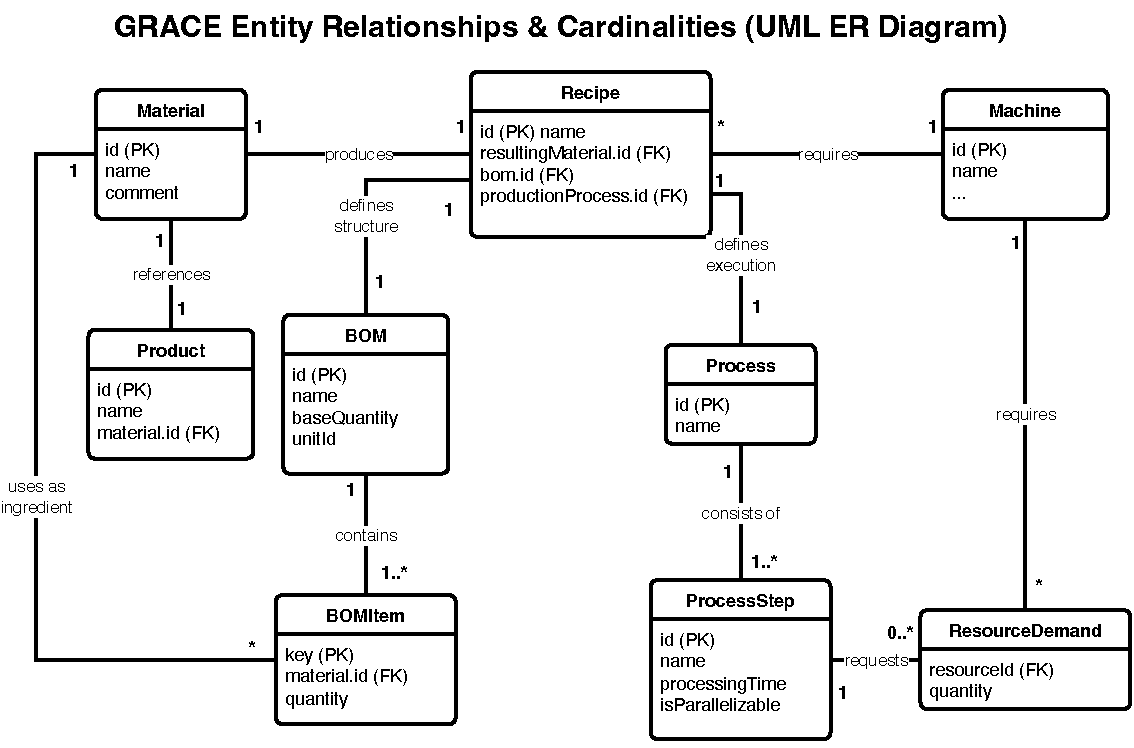
\includegraphics[width=0.9\textwidth]{@Bilder/ER_UML_Card.pdf}
    \caption{Entity-Relationship-Diagramm der GRACE-Konfigurationsentitäten. Zeigt die Abhängigkeitskette von Basis-Entitäten (Materials, Machines) über referenzierende Entitäten (Products, BOMs, Processes) bis zur finalen Verknüpfung in Recipes. Kardinalitäten verdeutlichen die Komplexität der referenziellen Integrität. Materials und Machines sind unabhängig. Products und BOMs referenzieren Materials mit unterschiedlicher Semantik (1:1 vs 1:n). Processes können mehrere Maschinen gleichzeitig beanspruchen (n:m). Recipes erfordern exakte Übereinstimmung dreier unabhängiger Entitäten (1:1:1).}
    \label{fig:grace_er_model}
\end{figure}

\noindent Diese Kardinalitäten optimierten die System-Prompt-Entwicklung durch drei Mechanismen: (1) \textbf{Explizite Constraint-Formulierung} - Jede Kardinalität wurde als CRITICAL-Rule in den System Prompt integriert (z.\,B. \glqq Product.material.id references the product itself, NOT ingredients\grqq{}), was das LLM von impliziter Inferenz auf explizite Regelanwendung lenkte. (2) \textbf{Kontextuelle Beispiele mit Negativfällen} - Für jede Kardinalität wurden verallgemeinerte Beispiele aus dem Entity Mapping Workbook mit expliziten Fehlerfällen ergänzt (z.\,B. \url{white-paste} vs \url{titanium-dioxide}), was die Fehlerrate bei Product-Material-Referenzen um 80\% reduzierte. (3) \textbf{Dependency-Chain-Awareness} - Die hierarchische Abhängigkeitskette (Materials/Machines $\rightarrow$ Products/BOMs/Processes $\rightarrow$ Recipes) wurde in der Session-Context-Generierung berücksichtigt, sodass bei Recipe-Erstellung bereits alle referenzierbaren IDs bekannt waren und das LLM keine nicht-existierenden Referenzen halluzinieren konnte.

\paragraph{Problem 1: Falsche Referenz-Kardinalitäten}

Das LLM setzte Entities nicht in korrekte Verhältnisse zueinander:

\begin{itemize}
    \item \textbf{Recipe → Material/BOM/Process (n:1:1:1):} Recipes referenzierten häufig nicht-existierende IDs oder verwendeten inkonsistente ID-Namenskonventionen.

    \item \textbf{Product → Material (1:1):} Das LLM interpretierte \glqq Product for White Paste\grqq{} fälschlicherweise als Referenz auf Zutaten (\url{titanium-dioxide}) statt auf das Produkt selbst (\url{white-paste}).
\end{itemize}

\paragraph{Lösung: Explizite Kardinalitäts-Modellierung mit Beispielen}

Die System-Prompt wurde erweitert um explizite Constraint-Formulierungen und verallgemeinerte Beispiele aus dem Entity Mapping Workbook:

\begin{minted}[fontsize=\footnotesize, breaklines]{text}
CRITICAL: Product.material.id references the product itself,
          NOT the ingredients.

Example: Product "White Pigment Paste"
{
  "id": "white-paste-prod",
  "name": "White Pigment Paste",
  "material": {"id": "white-paste"}  // NOT "titanium-dioxide"!
}
\end{minted}

\noindent Diese kontextuellen Beispiele (im Sinne von \cite{openai:sora_android2025}) führten zu deutlich besseren Ergebnissen als abstrakte Regeln allein.

\paragraph{Problem 2: Arithmetische Fehler}

Das LLM machte systematische Fehler bei arithmetischen Berechnungen:

\begin{itemize}
    \item \textbf{BOM baseQuantity:} Die Summe der \url{item.quantity}-Werte stimmte nicht mit \url{baseQuantity} überein (z.\,B. 30 + 60 + 10 = 110 statt 100).

    \item \textbf{Mengenverhältnisse inkonsistent:} BOM-Items ergaben zusammen nicht die korrekte Product-Menge.
\end{itemize}

\noindent Diese Fehler konnten durch Prompt-Engineering allein nicht gelöst werden, da sie fundamentale LLM-Schwächen bei arithmetischen Operationen darstellen.

\subsubsection{Phase 6: Implementierung als Master Creator Tool mit Validierungs-Layer}

Nach Stabilisierung der Unified Prompt wurde das vollständige Master Creator Tool implementiert:

\paragraph{Frontend-Implementierung (HTML/CSS/JavaScript)}

\begin{itemize}
    \item \textbf{HTML:} Chat-Interface, Entity-Listen (farbcodiert nach Typ), Validierungs-Sidebar, Export-Buttons
    \item \textbf{CSS:} Farbcodierung der 6 Entity-Typen (Materials: Lila, Machines: Pink, Products: Blau, Processes: Pink/Gelb, BOMs: Teal, Recipes: Pink), Responsive Design
    \item \textbf{JavaScript:} Ollama-API-Kommunikation, JSON-Extraktion aus Markdown-Code-Blocks, Session-Context-Management (localStorage), Validierungs-Engine
\end{itemize}

\paragraph{JavaScript Validierungs- und Korrektur-Layer}

Um die arithmetischen LLM-Schwächen deterministisch zu kompensieren, wurde ein JavaScript-Layer implementiert (siehe Abschnitt~\ref{sec:Validierung}), der:

\begin{itemize}
    \item BOM \url{baseQuantity} automatisch korrigiert (Summe aller \url{item.quantity})
    \item Referenzielle Integrität validiert (alle referenzierten IDs existieren)
    \item Fehlende Dependencies automatisch erstellt (Auto-Creation von Materials bei Products/BOMs)
    \item Validierungsergebnisse farbcodiert im Chat visualisiert
\end{itemize}

\subsubsection{Finale System-Prompt-Struktur}

Die finale Master Creator System-Prompt kombiniert alle Erkenntnisse aus den 5 Entwicklungsphasen:

\begin{minted}[fontsize=\footnotesize, breaklines]{text}
You are an APS Configuration Assistant.

STEP 1: DETECT ENTITY TYPE - CHECK KEYWORDS IN THIS ORDER!

1. If user says "produce" or "manufacture" -> PRODUCT
2. If user says "machine", "mixer", "pump" -> MACHINE
3. If user describes steps with "->" or "process" -> PROCESS
4. If user says "bom" or lists ingredients -> BOM
5. If user says "recipe" -> RECIPE
6. Otherwise -> MATERIAL

CRITICAL: "I produce X" = PRODUCT, not material!

[...Entity-Typen 1-6 mit JSON-Strukturen, Defaults, Beispielen...]

UNIVERSAL RULES FOR ALL ENTITY TYPES:
1. NEVER invent or guess data
2. Use EXACT names/values from user's message
3. Use defaults for missing fields
4. IDs are lowercase-with-hyphens
5. MULTIPLE ENTITIES: Create SEPARATE code blocks for each
\end{minted}

\noindent Die Prompt umfasst ca. 400 Zeilen und enthält für jeden Entity-Typ: JSON-Struktur, kritische Constraints, verallgemeinerte Beispiele, Defaults. Sie ist im Anhang hinterlegt unter \cite{anhang:system_prompt}.


\subsection{BPMN-Prozessmodelle}
\label{sec:BPMN}

Die drei Konfigurationsprozessvarianten (v1a: manuell, v1b: Importer-basiert, v2: LLM-gestützt) werden als BPMN-Diagramme (Business Process Model and Notation) modelliert. BPMN ermöglicht die standardisierte Visualisierung von Geschäftsprozessen mit Fokus auf Rollen (Lanes), Aktivitäten, Kontrollfluss und Iterationen.

\subsubsection{Prozessmodellierungs-Methodik}

Die BPMN-Diagramme nutzen folgende Notationselemente (gemäß BPMN 2.0):

\begin{itemize}
    \item \textbf{Lanes (Swimlanes):} Vertikale Bereiche für Akteure (Kunde, Konfigurationsteam, GRACE System, Master Creator/LLM)
    \item \textbf{Start-Event:} Grüner Kreis (Prozessbeginn)
    \item \textbf{End-Event:} Roter Kreis (Prozessende)
    \item \textbf{Tasks/Activities:} Abgerundete Rechtecke (Aktivitäten/Aufgaben)
    \item \textbf{Gateways:} Rauten (Entscheidungspunkte: \glqq Passt?\grqq{}, \glqq OK?\grqq{}, \glqq Fehler?\grqq{})
    \item \textbf{Sequence Flow:} Pfeile (Kontrollfluss zwischen Aktivitäten)
    \item \textbf{Message Flow:} Gestrichelte Pfeile (Kommunikation zwischen Lanes)
\end{itemize}

\noindent Farbcodierung visualisiert Aktivitätstypen: Gelb für zeitintensive Kernaktivitäten, Rot für Fehlerbehandlung, Grün für Abschlussaktivitäten.

\subsubsection{Prozessvariante v1a: Vollständig manuelle Konfiguration}

Abbildung~\ref{fig:bpmn_v1a} zeigt den manuellen Konfigurationsprozess über die GRACE UI mit einer Gesamtdurchlaufzeit von ca. 2 Monaten. Die unskalierte Darstellung ist im Anhang hinterlegt unter \cite{anhang:bpmn_v1a_full}.

\begin{figure}[h]
\centering
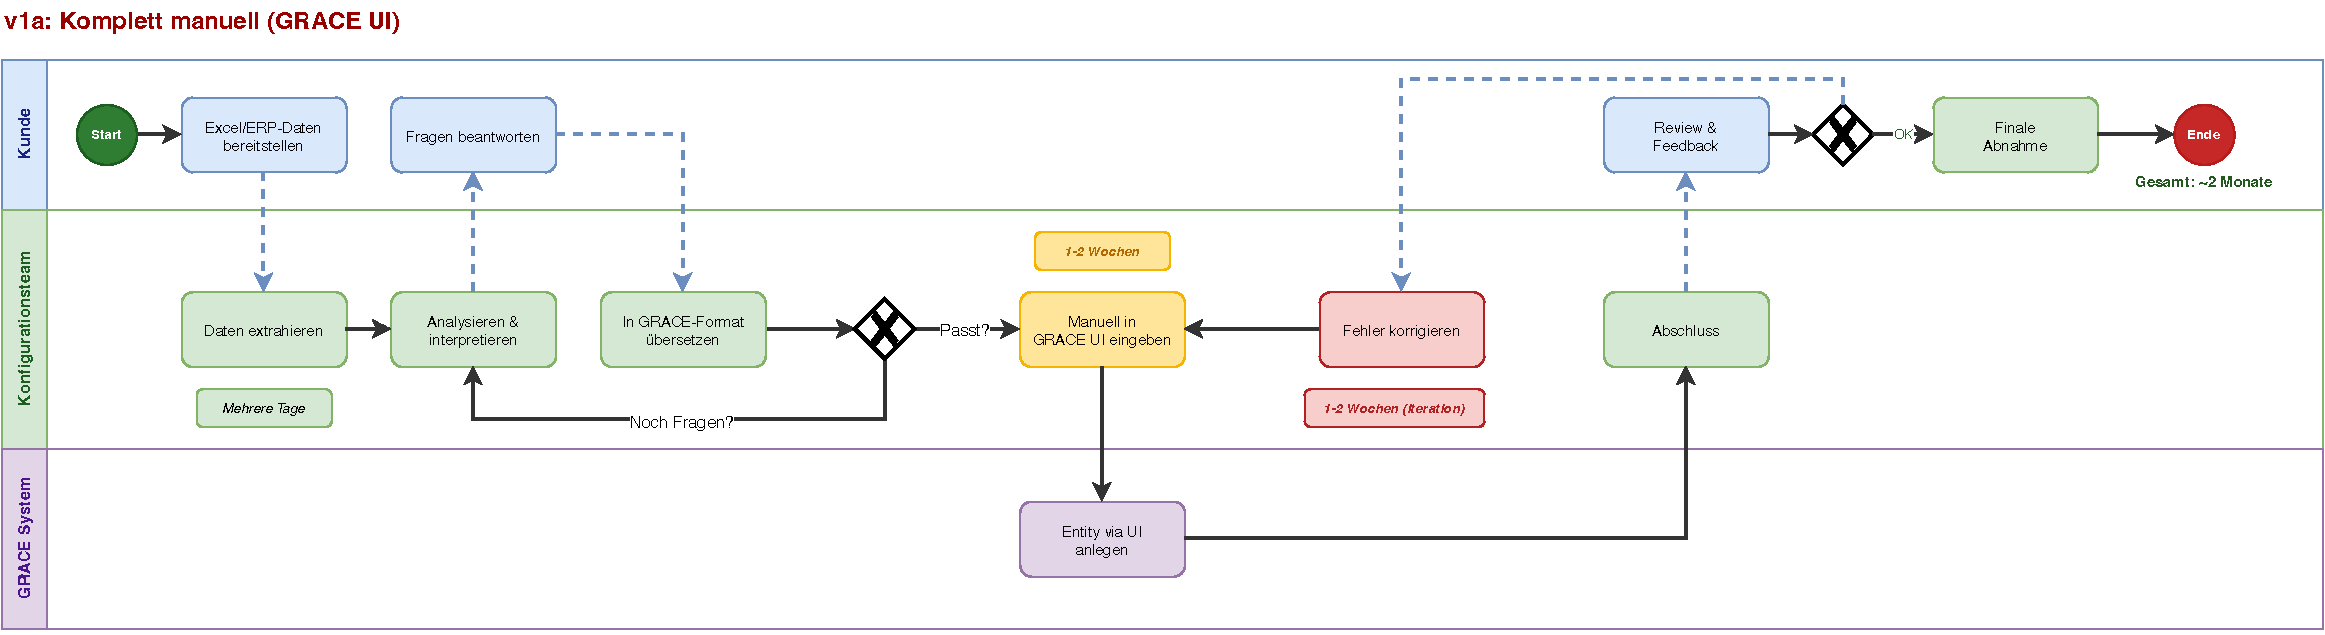
\includegraphics[width=\textwidth]{@Bilder/bpmn-v1a.pdf}
\caption{BPMN-Diagramm: Prozessvariante v1a - Vollständig manuelle Konfiguration (Gesamt: ca. 2 Monate)}
\label{fig:bpmn_v1a}
\end{figure}

\paragraph{Prozessschritte Konfigurationsteam}

\begin{enumerate}
    \item \textbf{Daten extrahieren} (mehrere Tage): Excel- oder ERP-Exportdateien vom Kunden entgegennehmen und relevante Produktionsdaten (Materialien, Maschinen, Rezepturen) extrahieren

    \item \textbf{Analysieren \& interpretieren:} Kundenspezifische Terminologie verstehen, Produktionsprozesse rekonstruieren, fehlende Informationen identifizieren (Gateway: \glqq Noch Fragen?\grqq{} → zurück zu Kunde)

    \item \textbf{In GRACE-Format übersetzen:} Daten in GRACE-Entitätsstrukturen mappen (Materials, Machines, Products, Processes, BOMs, Recipes)

    \item \textbf{Manuell in GRACE UI eingeben} (1-2 Wochen): Jede Entity einzeln über Web-Interface erstellen, Felder ausfüllen, Referenzen manuell verknüpfen (Gateway: \glqq Passt?\grqq{})

    \item \textbf{Fehler korrigieren} (1-2 Wochen, Iteration): Nach GRACE-Validierung: Fehlerhafte Referenzen korrigieren, fehlende Defaults nachtragen, Zeiteinheiten anpassen (iterative Schleife)

    \item \textbf{Abschluss:} Konfiguration an Kunde übergeben (Review \& Feedback → Finale Abnahme)
\end{enumerate}

\paragraph{Charakteristika}

\begin{itemize}
    \item \textbf{Hohe Parallelität:} Kunde und Konfigurationsteam iterieren häufig (\glqq Fragen beantworten\grqq{} <-> \glqq Analysieren \& interpretieren\grqq{})
    \item \textbf{Fehleranfällig:} Manuelle Eingabe führt zu Tippfehlern, inkonsistenten IDs, fehlenden Referenzen
    \item \textbf{GRACE System passiv:} Nur UI-Bereitstellung, keine Automatisierung
    \item \textbf{Lange Fehlerkorrektur-Iteration:} 1-2 Wochen pro Iterationsschleife
\end{itemize}

\subsubsection{Prozessvariante v1b: Konfiguration mit Importer}

Abbildung~\ref{fig:bpmn_v1b} zeigt den automatisierten Import-Prozess mit einer Gesamtdurchlaufzeit von ca. 3,5 Wochen. Die unskalierte Darstellung ist im Anhang
hinterlegt unter \cite{anhang:bpmn_v1b_full}

\begin{figure}[h]
\centering
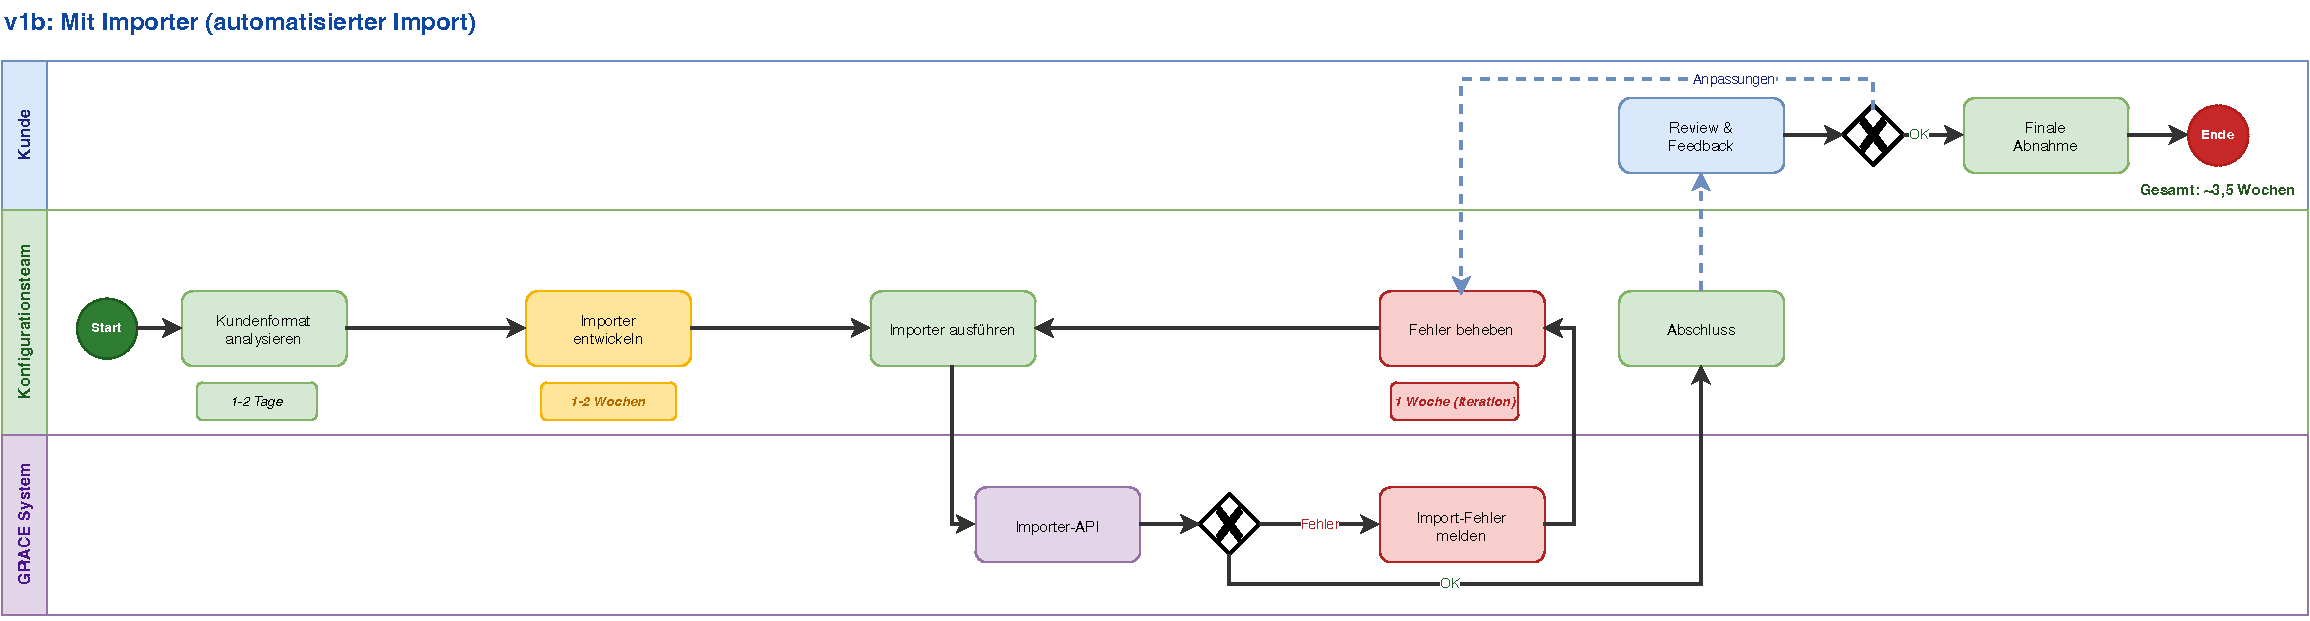
\includegraphics[width=\textwidth]{@Bilder/bpmn-v1b.pdf}
\caption{BPMN-Diagramm: Prozessvariante v1b - Konfiguration mit Importer (Gesamt: ca. 3,5 Wochen)}
\label{fig:bpmn_v1b}
\end{figure}

\paragraph{Prozessschritte Konfigurationsteam}

\begin{enumerate}
    \item \textbf{Kundenformat analysieren} (1-2 Tage): Struktur der Kundendaten verstehen (Excel-Spalten, ERP-Felder, CSV-Format)

    \item \textbf{Importer entwickeln} (1-2 Wochen): Projektspezifischen Importer programmieren (Python/JavaScript), Mapping-Logik implementieren, GRACE-API-Integration

    \item \textbf{Importer ausführen:} Skript auf Kundendaten laufen lassen → GRACE-Importer-API aufrufen

    \item \textbf{Fehler beheben} (1 Woche, Iteration): Import-Fehler (fehlende Felder, falsche Datentypen, broken references) analysieren und Importer-Code anpassen (iterative Schleife mit GRACE System: \glqq Import-Fehler melden\grqq{})

    \item \textbf{Abschluss:} Finale Konfiguration validieren und an Kunde übergeben
\end{enumerate}

\paragraph{Charakteristika}

\begin{itemize}
    \item \textbf{Initiale Entwicklungszeit dominiert:} Importer-Entwicklung (1-2 Wochen) ist größter Aufwand
    \item \textbf{Wiederverwendbarkeit begrenzt:} Jeder Kunde hat individuelles Datenformat → projektspezifische Importer-Anpassung
    \item \textbf{GRACE System aktiv:} Importer-API validiert Daten, meldet Fehler zurück
    \item \textbf{Reduzierte Iteration:} Weniger Kunden-Interaktion als v1a, aber Debugging-Iterationen zwischen Code und API
\end{itemize}

\subsubsection{Prozessvariante v2: LLM-gestützte Konfiguration mit Master Creator}

Abbildung~\ref{fig:bpmn_v2} zeigt den durch Master Creator automatisierten Prozess. Die unskalierte Darstellung ist im Anhang hinterlegt unter \cite{anhang:bpmn_v2_full}.

\begin{figure}[h]
\centering
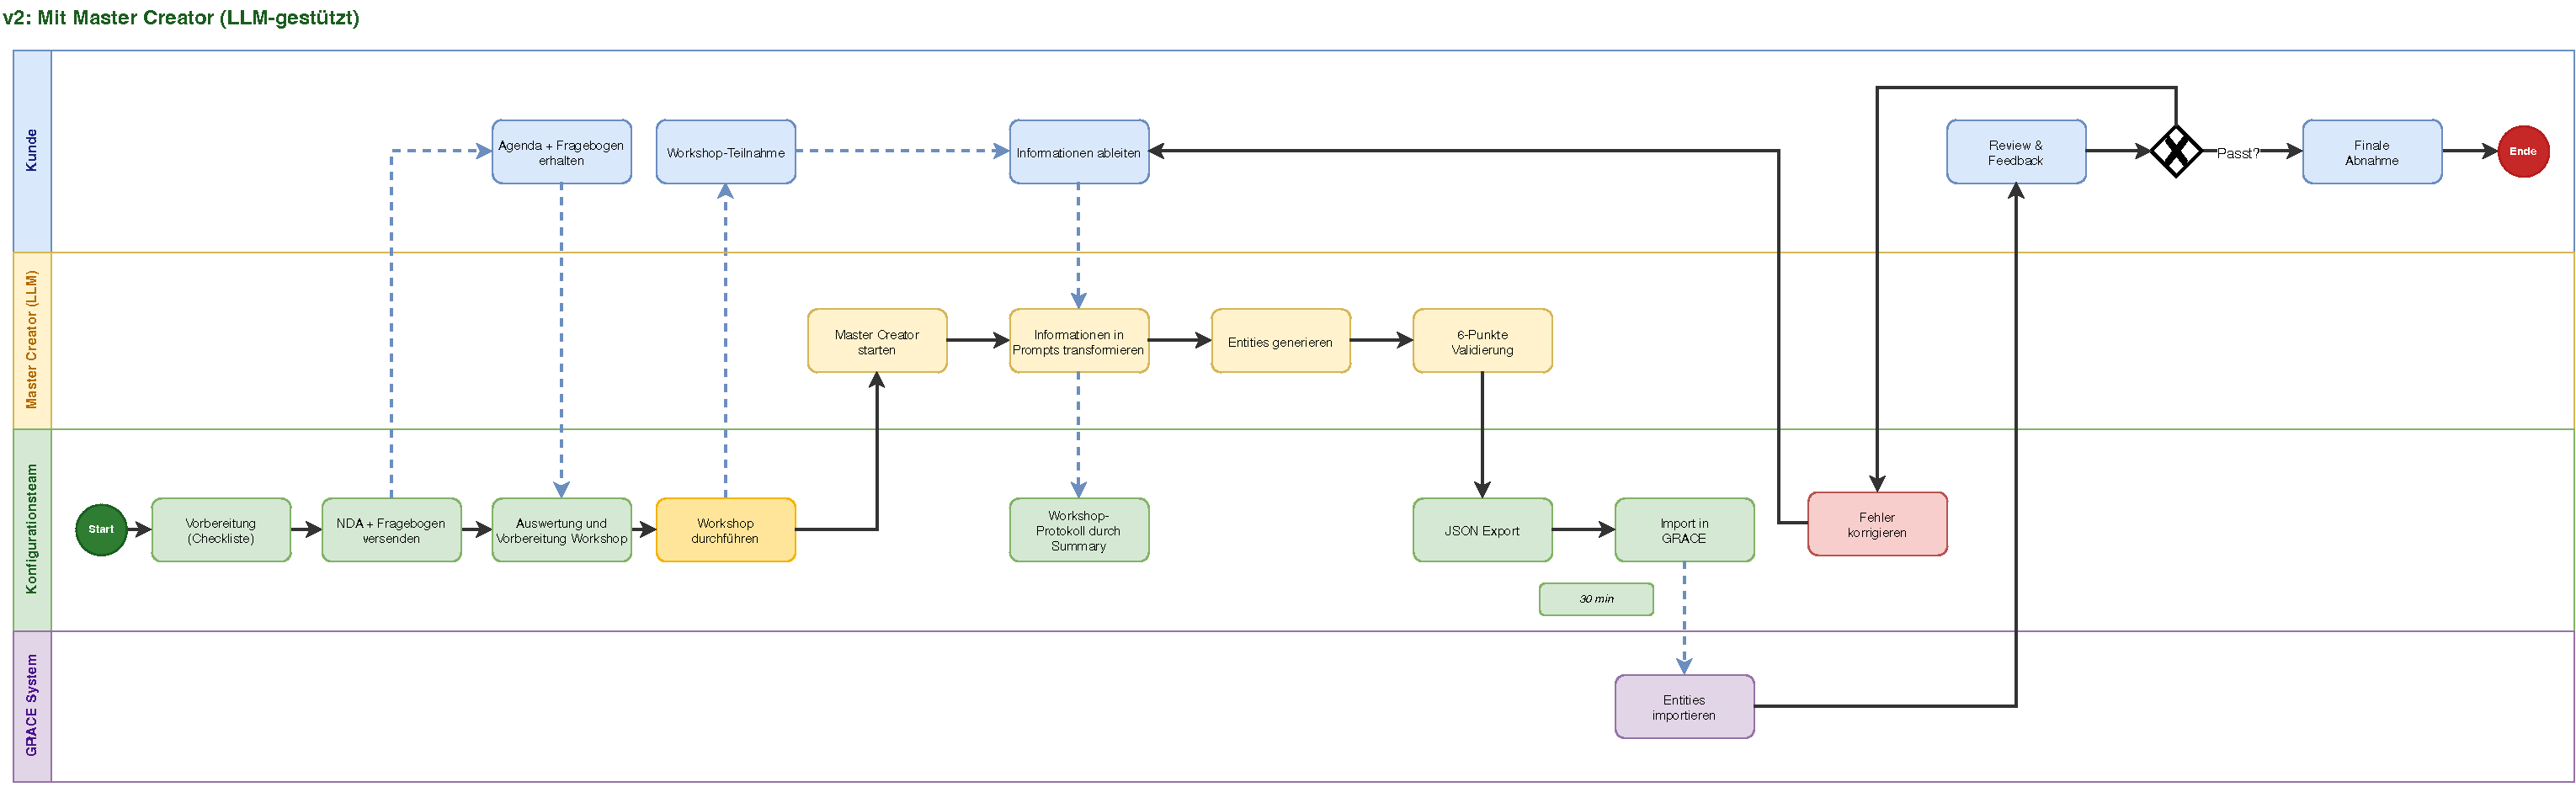
\includegraphics[width=\textwidth]{@Bilder/bpmn-v2.pdf}
\caption{BPMN-Diagramm: Prozessvariante v2 - LLM-gestützte Konfiguration}
\label{fig:bpmn_v2}
\end{figure}

\paragraph{Prozessschritte Konfigurationsteam}

\begin{enumerate}
    \item \textbf{Vorbereitung (Checkliste):} SOP 01 (Kundenworkshop) vorbereiten, Agenda erstellen

    \item \textbf{NDA + Fragebogen versenden:} GRACE Onboarding Fragebogen (Kompaktversion, 15 Fragen) und NDA an Kunde senden

    \item \textbf{Auswertung und Vorbereitung Workshop:} Fragebogen-Antworten analysieren, Workshop-Schwerpunkte identifizieren

    \item \textbf{Workshop durchführen:} Strukturiertes Interview gemäß SOP 01 (6 Themenblöcke: Grundlagen, IT-Landschaft, Produktionsdetails, Planung, Restriktionen, Next Steps)

    \item \textbf{Import in GRACE} (30 min): Generierte JSONs über GRACE-UI importieren gemäß SOP 03

    \item \textbf{Fehler korrigieren:} Validierungsfehler beheben (typischerweise 3-5 Fehler aus 6-Punkte-Checkliste)

    \item \textbf{Abschluss:} Finale Konfiguration an Kunde übergeben
\end{enumerate}

\paragraph{Prozessschritte Master Creator (LLM)}

\begin{enumerate}
    \item \textbf{Master Creator starten:} Ollama-Server und Master Creator UI starten (localhost:9000)

    \item \textbf{Informationen in Prompts transformieren:} Workshop-Protokoll in natürlichsprachige Prompts übersetzen (z.\,B. \glqq I need Titanium Dioxide, PEG 400, and Tego\grqq{})

    \item \textbf{Entities generieren:} LLM generiert JSON-Strukturen für alle 6 Entity-Typen basierend auf System-Prompt und Session-Context

    \item \textbf{6-Punkte Validierung:} JavaScript-Validierungsschicht prüft Vollständigkeit, ID-Konsistenz, Zeiteinheiten, BOM baseQuantity, Product Material, ID-Duplikate

    \item \textbf{JSON Export:} Validierte JSONs einzeln oder kombiniert exportieren
\end{enumerate}

\paragraph{Prozessschritte Kunde}

Im Gegensatz zu v1a/v1b erhält der Kunde strukturierte Vorbereitung:

\begin{enumerate}
    \item \textbf{Agenda + Fragebogen erhalten:} Klare Erwartungshaltung, Vorbereitung auf Workshop-Themen

    \item \textbf{Workshop-Teilnahme:} Aktive Mitwirkung statt passiver Datenbereitstellung

    \item \textbf{Informationen ableiten:} Kunde kann aus Workshop-Summary lernen (Chat-Summarization als Wissensdokument)
\end{enumerate}

\paragraph{Charakteristika}

\begin{itemize}
    \item \textbf{Neue Lane: Master Creator (LLM):} Explizite Modellierung der LLM-Aktivitäten als eigenständiger Akteur

    \item \textbf{Frontloading:} Vorbereitung (Fragebogen, Workshop-Planung) dominiert, nicht Implementierung

    \item \textbf{Minimale Iteration:} Fehlerkorrektur-Schleife deutlich kleiner als v1a/v1b

    \item \textbf{Strukturierte Wissenserfassung:} Workshop folgt SOP 01 (6 Themenblöcke), nicht ad-hoc Datensammlung

    \item \textbf{Chat-Summarization als Dokumentation:} Workshop-Protokoll automatisch generiert (\glqq Workshop-Protokoll durch Summary\grqq{})

    \item \textbf{Kurzer Import:} GRACE-Import dauert nur ca. 30 Minuten (im Vergleich zu Wochen bei v1a/v1b)
\end{itemize}

\subsubsection{Strukturelle Prozessunterschiede}

Die drei Varianten unterscheiden sich fundamental in ihrer Prozessstruktur:

\paragraph{Sequentialität vs. Parallelität}

\begin{itemize}
    \item \textbf{v1a:} Hohe Parallelität zwischen Kunde und Konfigurationsteam (viele Message Flows)
    \item \textbf{v1b:} Sequentieller Ablauf (Importer-Entwicklung entkoppelt von Kunden-Interaktion)
    \item \textbf{v2:} Frontloaded Parallelität (Workshop + Master Creator), dann sequentiell
\end{itemize}

\paragraph{Fehlerbehandlung}

\begin{itemize}
    \item \textbf{v1a:} Lange iterative Schleife (\glqq Fehler korrigieren\grqq{} 1-2 Wochen <-> \glqq Manuell in GRACE UI eingeben\grqq{} 1-2 Wochen)
    \item \textbf{v1b:} Iterative Schleife zwischen Konfigurationsteam und GRACE System (\glqq Fehler beheben\grqq{} 1 Woche <-> \glqq Import-Fehler melden\grqq{})
    \item \textbf{v2:} Kurze Fehlerkorrektur-Schleife nach Import (6-Punkte-Validierung reduziert Fehlerquellen präventiv)
\end{itemize}

\paragraph{Automatisierungsgrad}

\begin{itemize}
    \item \textbf{v1a:} Keine Automatisierung (GRACE System nur UI-Provider)
    \item \textbf{v1b:} Partielle Automatisierung (Importer-API, aber projektspezifische Entwicklung erforderlich)
    \item \textbf{v2:} Hohe Automatisierung (LLM-Generierung, JavaScript-Validierung, Auto-Correction, Auto-Creation)
\end{itemize}

